\documentclass[letterpaper]{article}
\usepackage[margin=1in]{geometry}
\usepackage[utf8]{inputenc}
\usepackage{textcomp}
\usepackage{amssymb}
\usepackage{natbib}
\usepackage{graphicx}
\usepackage{gensymb}
\usepackage{amsthm, amsmath, mathtools}
\usepackage[dvipsnames]{xcolor}
\usepackage{enumerate}
\usepackage{mdframed}
\usepackage[most]{tcolorbox}
\usepackage{csquotes}
% https://tex.stackexchange.com/questions/13506/how-to-continue-the-framed-text-box-on-multiple-pages

\tcbuselibrary{theorems}

\newcommand{\R}{\mathbb{R}}
\newcommand{\Z}{\mathbb{Z}}
\newcommand{\N}{\mathbb{N}}
\newcommand{\Q}{\mathbb{Q}}
\newcommand{\C}{\mathbb{C}}
\newcommand{\code}[1]{\texttt{#1}}
\newcommand{\mdiamond}{$\diamondsuit$}
\newcommand{\PowerSet}{\mathcal{P}}
\newcommand{\Mod}[1]{\ (\mathrm{mod}\ #1)}
\DeclareMathOperator{\lcm}{lcm}

%\newtheorem*{theorem}{Theorem}
%\newtheorem*{definition}{Definition}
%\newtheorem*{corollary}{Corollary}
%\newtheorem*{lemma}{Lemma}
\newtheorem*{proposition}{Proposition}


\newtcbtheorem[number within=section]{theorem}{Theorem}
{colback=green!5,colframe=green!35!black,fonttitle=\bfseries}{th}

\newtcbtheorem[number within=section]{definition}{Definition}
{colback=blue!5,colframe=blue!35!black,fonttitle=\bfseries}{def}

\newtcbtheorem[number within=section]{corollary}{Corollary}
{colback=yellow!5,colframe=yellow!35!black,fonttitle=\bfseries}{cor}

\newtcbtheorem[number within=section]{lemma}{Lemma}
{colback=red!5,colframe=red!35!black,fonttitle=\bfseries}{lem}

\newtcbtheorem[number within=section]{example}{Example}
{colback=white!5,colframe=white!35!black,fonttitle=\bfseries}{def}

\newtcbtheorem[number within=section]{note}{Important Note}{
        enhanced,
        sharp corners,
        attach boxed title to top left={
            xshift=-1mm,
            yshift=-5mm,
            yshifttext=-1mm
        },
        top=1.5em,
        colback=white,
        colframe=black,
        fonttitle=\bfseries,
        boxed title style={
            sharp corners,
            size=small,
            colback=red!75!black,
            colframe=red!75!black,
        } 
    }{impnote}
\usepackage[utf8]{inputenc}
\usepackage[english]{babel}
\usepackage{fancyhdr}
\usepackage[hidelinks]{hyperref}

\fancypagestyle{noheader}{
  \fancyhf{}% Clear header/footer
  \renewcommand{\headrulewidth}{0pt}% No header rule
  \rfoot{\thepage}
} 

\pagestyle{fancy}
\fancyhf{}
\rhead{CSE 131}
\chead{June 9th, 2023}
\lhead{Course Notes}
\rfoot{\thepage}

\setlength{\parindent}{0pt}

\begin{document}

\begin{titlepage}
    \begin{center}
        \vspace*{1cm}
            
        \Huge
        \textbf{CSE 131 Notes}
            
        \vspace{0.5cm}
        \LARGE
        Compiler Construction
            
        \vspace{1.5cm}
            
        \vfill
            
        Spring 2023\\
        Taught by Professor Joe Politz
    \end{center}
\end{titlepage}

\pagenumbering{gobble}

\newpage 

\pagenumbering{gobble}
\begingroup
    \renewcommand\contentsname{Table of Contents}
    \tableofcontents
\endgroup

\newpage
\pagenumbering{arabic}


\section{Introduction to Compilers}
Some examples of compilers we've used in this class include 
\begin{center}
    \begin{tabular}{|c|c|}
        \hline 
        \code{gcc} & C to binary  \\ 
        \code{g++} & C++ to binary  \\ 
        \code{rustc} & Rust to binary \\ 
        \code{javac} & Java to JVM bytecode \\ 
        \code{ghc} & Haskell to Haskell magic \\ 
        \code{tsc} & TypeScript to JavaScript \\ 
        \hline 
    \end{tabular}
\end{center}
Essentially, a compiler takes some program and produces an output program, one that is easier for us to run in some environment. In this course, we're going to create a compiler \code{ucsdc} that takes in \code{snek} files and will produce \code{x86\_64} binaries.

\bigskip 

To be more specific, our compiler should do the following: given a \code{.snek} text file, 
\begin{itemize}
    \item parse\footnote{Known to be very boring.} the text into an abstract syntax tree (AST), 
    \begin{mdframed}
        (Example.) For example, consider the following Java class. 
\begin{verbatim}
class Pt {
    int x; 
    int y; 
}\end{verbatim}
        Its AST representation might look like 
        \begin{center}
            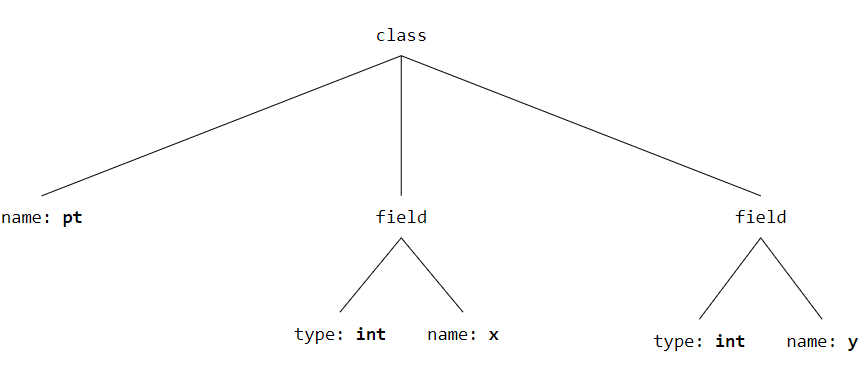
\includegraphics[scale=0.8]{assets/ast.png}
        \end{center}
    \end{mdframed}
    \item and either 
    \begin{itemize}
        \item generates assembly (or some other output program), or 
        \item generate an error message.
    \end{itemize}
\end{itemize}
We are \underline{not} interested in generating the most optimized assembly, just that it works. Most of the time spent in this course will be on the code generating part (i.e., from AST to assembly). Towards the \emph{end} of the course, we'll work with libraries/runtime.

\subsection{S-Expressions}
We'll be using s-expressions to represent our program's source code. That is, each \code{snek} file will contain s-expressions. S-expressions are defined as either 
\begin{itemize}
    \item An \textbf{atom} of the form $x$, or 
    \item An \textbf{expression} of the form $(x \quad y)$, where $x$ and $y$ are s-expressions. 
\end{itemize}
For example, \code{(sub1 2)} is an expression with two atoms, \code{sub1} and \code{2}. 

\subsubsection{The \code{sexp} Crate}
Most programming language will have a parser for s-expressions. In Rust, we have the \code{sexp} crate. This crate has the following \code{enum}s\footnote{In Rust, \code{enum}s are algebraic data types.}:
\begin{itemize}
    \item A \code{Sexp} enum, representing either an \code{Atom} or a vector of s-expressions. Vectors of s-expressions will contain two elements (since an expression has the form $(x \quad y)$, which has two expressions). 
    \begin{verbatim}
pub enum Sexp {
    Atom(Atom),
    List(Vec<Sexp>),
}
    \end{verbatim}

    \item An \code{Atom} enum, representing one of three different types of atoms: a \code{String}, \code{i64} (64-bit signed integer), or \code{f64} (double-precision float). 
    \begin{verbatim}
pub enum Atom {
    S(String),
    I(i64),
    F(f64)
}\end{verbatim}
\end{itemize}

\begin{mdframed}
    (Exercise.) Why is \code{Vec<Box<Sexp>>} or \code{Box<Vec<Sexp>>} not used in the \code{enum} definitions above? 

    \begin{mdframed}
        Remember that the reason why something like 
        \begin{verbatim}
enum Expr {
    Num(i32),
    Add1(Expr),
    Sub1(Expr)
}\end{verbatim}
        wouldn't work is because \code{Expr}, as a recursive type, could have infinite size. That is, we could nest \emph{many} \code{Expr}s, and since this value could theoretically continue infinitely, so we don't know how much space this recursive type needs. However, \code{Box<T>} is a pointer type that allocates memory on the heap. \code{Box<T>} has a \emph{fixed} size, so Rust is fine if we have \code{Box<Expr>}. 

        \bigskip

        The reason why we \emph{don't} need \code{Vec<Box<Sexpr>>} or \code{Box<Vec<Sexpr>>} in the above \code{enum}s is because \code{Vec<T>} allocates to the heap (when you add any elements; a vector created initially with no elements does not allocate). In other words, think of \code{Vec<T>} as being a resizable \code{Box<T>}. More accurately, a \code{Vec<T>} is a fixed-size type with a reference to variable-sized heap data.
    \end{mdframed}
\end{mdframed}


\begin{mdframed}
    (Exercise.) Represent the following s-expression in Rust: 
    \begin{verbatim}
        (sub1 (sub1 (add1 73)))\end{verbatim}
    
    \begin{mdframed}
        First, the s-expression itself is roughly similar to a tree, where each \emph{atom} is a leaf node and each \emph{list} is another s-expression. In any case, we can roughly structure the above s-expression like so: 
        \begin{verbatim}
(               // List
    sub1            // Atom 
    (               // List 
        sub1            // Atom 
        (               // List 
            add1            // Atom 
            73              // Atom 
        )
    )
) \end{verbatim}
        In other words, we have a list whose elements are an \emph{atom} and another \emph{list}. With this in mind, the Rust form is
        \begin{verbatim}
List(vec![
    Atom(S("sub1")),
    List(vec![
        Atom(S("sub1")),
        List(vec![
            Atom(S("add1")),
            Atom(I(73))
        ])
    ])
])\end{verbatim}
    \end{mdframed}
\end{mdframed}

\subsection{From S-Expressions to Rust Code}
Given some s-expression string, we can use the above crate to convert the s-expression into a Rust object. However, this Rust object itself doesn't give us much information aside from how the s-expression is structured. We want to turn this Rust object into another Rust object representing the actual expressions (i.e., an abstract syntax tree). We can use the Rust structure to represent our code: 
\begin{verbatim}
enum Expr {
    Num(i32),
    Add1(Box<Expr>),
    Sub1(Box<Expr>),
}\end{verbatim}
So, given the \code{Sexp}, our s-expression representation in Rust, we can use the following function to parse this representation into an abstract syntax tree: 
\begin{verbatim}
fn parse_expr(s : &Sexp) -> Expr {
    match s {
        Sexp::Atom(I(n)) =>
            Expr::Num(i32::try_from(*n).unwrap()),
            Sexp::List(vec) =>
                match &vec[..] {
                    [Sexp::Atom(S(op)), e] if op == "add1" =>
                        Expr::Add1(Box::new(parse_expr(e))),
                    [Sexp::Atom(S(op)), e] if op == "sub1" =>
                        Expr::Sub1(Box::new(parse_expr(e))),
                    _ => panic!("parse error")
	            },
        _ => panic!("parse error")
    }
}\end{verbatim}

\begin{mdframed}
    (Exercise.) Convert the s-expression representation in Rust of \code(sub1 (sub1 (add1 73))) to an \code{Expr} object. 

    \begin{mdframed}
        From the code above, our object might look like: 
        \begin{verbatim}
Expr::Sub1(
    Box::new(Expr::Sub1(
        Box::new(Expr::Add1(
            Box::new(
                Expr::Num(73)
            )
        ))
    ))
)\end{verbatim}
    \end{mdframed}
\end{mdframed}


\subsection{From AST to Assembly}
How do we convert our AST to assembly? We can use the following code to do this. 
\begin{verbatim}
fn compile_expr(e : &Expr) -> String {
    match e {
    	Expr::Num(n) => format!("mov rax, {}", *n),
    	Expr::Add1(subexpr) =>
            compile_expr(subexpr) + "\nadd rax, 1",
    	Expr::Sub1(subexpr) =>
            compile_expr(subexpr) + "\nsub rax, 1"
    }
}
\end{verbatim}

\begin{mdframed}
    (Exercise.) Convert \code(sub1 (sub1 (add1 73))) into assembly. 

    \begin{mdframed}
        The above code would produce the following assembly. 
        \begin{verbatim}
    mov rax, 73
    add rax, 1 
    sub rax, 1
    sub rax, 1\end{verbatim}
    \end{mdframed}
\end{mdframed}
\newpage
\section{Introduction to Binary Operations}

\begin{mdframed}
    Consider the following s-expression: \code{(sub1 (sub1 (add1 73)))}. Looking at the code discussed in the lecture handout, and assuming \code{main} runs, what does the stack and heap look like when \begin{verbatim}
        format!("mov rax, {}", *n)\end{verbatim} 
    evaluates? 

    \begin{mdframed}
        We'll take a look at the function calls of \code{compile\_expr(\&expr)}. First, note that Rust will store objects on the stack unless you allocate it on the heap. Recall, from the previous lecture, we have the AST representation 
                \begin{verbatim}
    Expr::Sub1(
        Box::new(Expr::Sub1(
            Box::new(Expr::Add1(
                Box::new(
                    Expr::Num(73)
                )
            ))
        ))
    )\end{verbatim}
        
        Our code initially calls \code{compile\_expr(\&expr)}, where \code{\&expr} is a reference to the above object. Note that the outer \code{Expr::Sub1} is in the stack, but the data in each of the \code{Enum}s will be allocated in the heap. In any case, after calling the function initially, it makes a recursive call with the argument being the held data of the inner object. This repeats until we reach the end (when we have the \code{Num}). 
        \begin{center}
            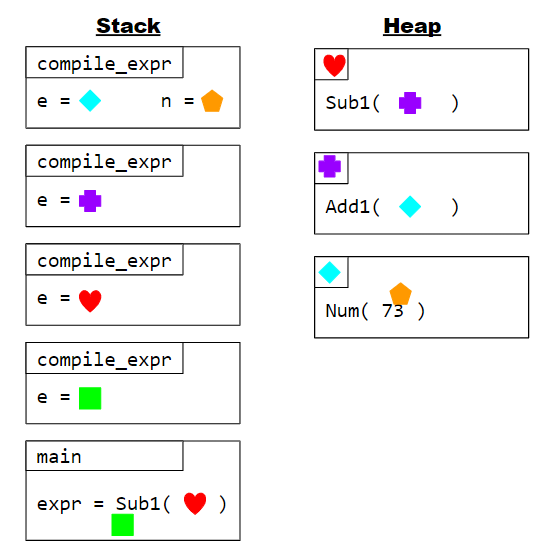
\includegraphics[scale=0.7]{assets/memory_diagram.png}
        \end{center}
    \end{mdframed}
\end{mdframed}

\subsection{Adding Binary Operation Support}
Let's suppose we want to add \code{(+ <expr> <expr>)} to our compiler. Our grammar for our language might look like 
\begin{verbatim}
    (*
        expr := <number> 
            | (add1 <expr>)
            | (sub1 <expr>)
            | (+ <expr> <expr>) 
    *)\end{verbatim}
The \code{Expr} \code{enum} might look like 
\begin{verbatim}
    enum Expr {
        Num(i32),
        Add1(Box<Expr>),
        Sub1(Box<Expr>),
        Plus(Box<Expr>, Box<Expr>),
    }\end{verbatim} 

\subsubsection{Creating the Parser}
Modifying the parser is simple. The \code{parse\_expr} function might look like 
\begin{verbatim}
pub fn parse_expr(s: &Sexp) -> Expr {
    match s {
        Sexp::Atom(I(n)) => Expr::Num(i32::try_from(*n).unwrap()),
        Sexp::List(list) => match &list[..] {
            [Sexp::Atom(S(op)), e] if op == "add1" => 
                Expr::Add1(Box::new(parse_expr(e))),
            [Sexp::Atom(S(op)), e] if op == "sub1" => 
                Expr::Sub1(Box::new(parse_expr(e))),
            [Sexp::Atom(S(op)), e] if op == "negate" => 
                Expr::Negate(Box::new(parse_expr(e))),
            [Sexp::Atom(S(op)), e1, e2] if op == "+" => {
                Expr::Add(Box::new(parse_expr(e1)), Box::new(parse_expr(e2)))
            }
            _ => panic!("parse error"),
        },
        _ => panic!("parse error"),
    }
}\end{verbatim}
Because we know that addition will always be of the form \code{(+ <expr> <expr>)}, we simply need to add a match condition to the inner \code{match} checking if the operation is \code{+}. 

\subsubsection{Modifying the Compiler: Part 1}
Suppose we update the \code{compile\_expr} function so it looks like  
\begin{verbatim}
    fn compile_expr(e: &Expr) -> String {
        match e {
            Expr::Num(n) => format!("mov rax, {}", *n),
            Expr::Add1(subexpr) => compile_expr(subexpr) + "\nadd rax, 1",
            Expr::Sub1(subexpr) => compile_expr(subexpr) + "\nsub rax, 1",
            Expr::Plus(e1, e2) => {
                let e1_instrs = compile_expr(e1);
                let e2_instrs = compile_expr(e2);
                e1_instrs + "\n mov rbx, rax" + &e2_instrs + "\n add rax, rbx"
            }
        }
    }\end{verbatim}

\begin{mdframed}
    (Exercise.) Using the above code for compiling, what is the assembly code generated after compiling the following code? What is the result of running the assembly? 
    \begin{enumerate}[(a)]
        \item \code{(+ (+ 100 30) 4)}
        \begin{mdframed}
            \begin{verbatim}
	mov rax, 500
	mov rbx, rax
	mov rax, 30
	mov rbx, rax
	mov rax, 9
	add rax, rbx
	add rax, rbx
	ret\end{verbatim}
            The result is \code{134}, as expected.
        \end{mdframed}

        \item \code{(+ 500 (+ 30 9))}
        \begin{mdframed}
            \begin{verbatim}
	mov rax, 500
	mov rbx, rax
	mov rax, 30
	mov rbx, rax
	mov rax, 9
	add rax, rbx
	add rax, rbx
	ret\end{verbatim}
            The result is \code{69}, which isn't what we were expecting. Notice how, in the second line, we effectively put \code{500} into \code{rbx}. In the fourth line, we overwrite \code{500} with \code{30}. In any case, this isn't what we were expecting, so option (a) will not work. 
        \end{mdframed}
    \end{enumerate}
\end{mdframed}

\subsubsection{Modifying the Compiler: Part 2}
Clearly, the first attempt at modifying the compiler didn't work. In fact, while this may work for simple addition operations, this won't work for more complex addition operations. 

\bigskip 

One solution is to essentially store important values in the stack, and then refer to the values in the stack when doing addition. This gives us the following code: 
\begin{verbatim}
    fn compile_expr(e: &Expr, si: i32) -> String {
        match e {
            Expr::Num(n) => format!("mov rax, {}", *n),
            Expr::Add1(subexpr) => compile_expr(subexpr, si) + "\nadd rax, 1",
            Expr::Sub1(subexpr) => compile_expr(subexpr, si) + "\nsub rax, 1",
            Expr::Plus(e1, e2) => {
                let e1_instrs = compile_expr(e1, si);
                let e2_instrs = compile_expr(e2, si + 1);
                let stack_offset = si * 8;
                format!("
                    {e1_instrs}
                    mov [rsp - {stack_offset}], rax
                    {e2_instrs}
                    add rax, [rsp - {stack_offset}]
                ")
            }
        }
    }\end{verbatim}
Some technical remarks: 
\begin{itemize}
    \item In our current setting, we do not need to allocate any memory. All we're doing is using is the stack memory, which the operating system gives us. The highest address is where the stack begins, and grows in decreasing address\footnote{All the operating system will do is, if we somehow use the entire stack space, we'll probably end up with a segfault.}. If we need to worry about creating a lot of objects or storing a lot of information on the heap, then we need to allocate memory. 
    
    \bigskip 

    Roughly speaking, this might look like 
    \begin{center}
        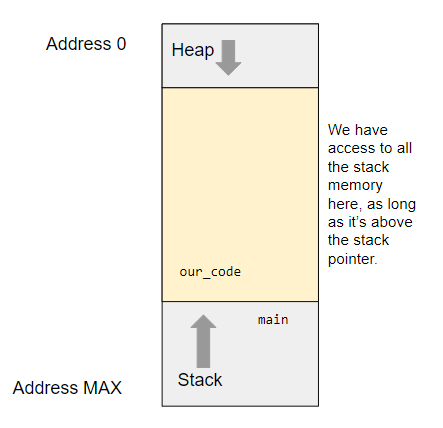
\includegraphics[scale=0.9]{assets/stack_vis.png}
    \end{center}
    \item \code{rsp} is the register representing the stack pointer. \code{rsp} points to the very bottom of the stack frame that we get to use for all of our generated code. 
    \item In the line \code{si * 8}, the \code{8} represents the size of a Word. This will be \code{8} for a 64-bit machine and \code{4} for a 32-bit machine. 
    \item The \code{si} parameter is the \textbf{stack index}. The stack index should initially be a small positive integer (e.g., 1 or 2). The stack index simply represents how deep in nested expressions or temporary variables we need to save. In this class, we'll prefer using the value \code{2} (i.e., 2 words up from where \code{rsp} is) because the bottom of the stack is where information like the return pointer (how we can use \code{ret}) is stored. We will generally use information one other word at the bottom of the stack.
\end{itemize}
In this sense, we'll initially call \code{compile\_expr} with the arguments \code{e} (our expression to compile) and \code{2} (the stack index).

\begin{mdframed}
    (Exercise.) Using the newly revised code for compiling, what is the assembly code generated after compiling the following code?
    \begin{verbatim}
        (+ (+ 100 50) 2)\end{verbatim}

    \begin{mdframed}
        Roughly speaking, the AST representation of the above code is 
        \begin{verbatim}
Plus(
    Plus(
        Num(100),
        Num(50)
    ),
    Num(2)
)\end{verbatim}

        Drawing out the recursion tree gives us 
        \begin{center}
            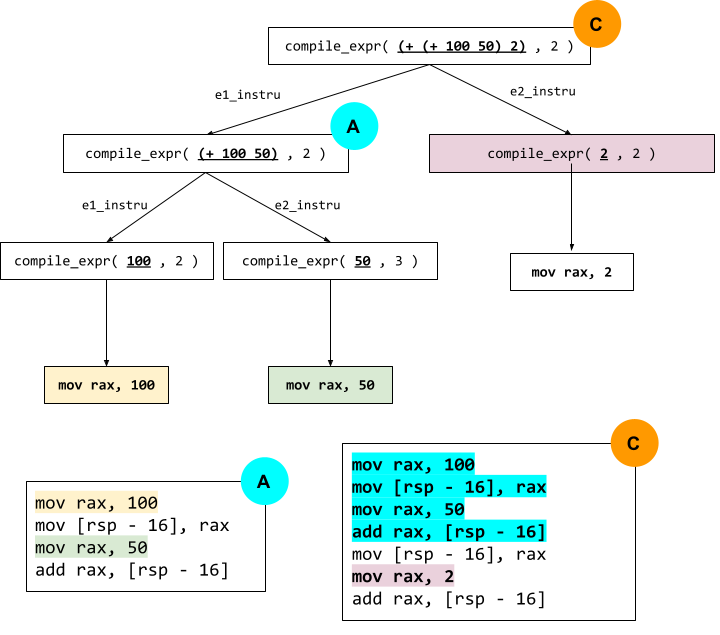
\includegraphics[scale=0.57]{assets/add_asm.png}
        \end{center}
        Note that the values passed in the function calls are intended to make things more clear, and will not compile otherwise. 
    \end{mdframed}
\end{mdframed}

\bigskip 

Here's the resulting assembly.
\begin{verbatim}
    mov rax, 100
    mov [rsp - 16], rax
    mov rax, 50 
    add rax, [rsp - 16]
    mov [rsp - 16], rax
    mov rax, 2
    add rax, [rsp - 16]\end{verbatim}
Suppose we run through each line of this assembly. This is what the resulting stack memory might look like: 
\begin{center}
    \begin{tabular}{p{2in}|p{4in}}
        Executed Line & Result After Running \\ 
        \hline 
        \code{mov rax, 100} & \raisebox{-\totalheight}{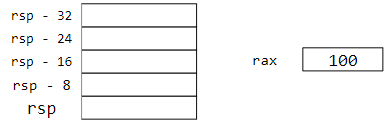
\includegraphics[scale=0.8]{assets/a1.png}} \\ 
        \hline 
        \code{mov [rsp - 16], rax} & \raisebox{-\totalheight}{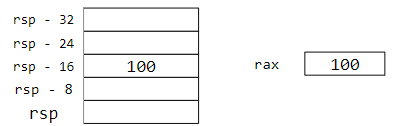
\includegraphics[scale=0.8]{assets/a2.png}} \\ 
        \hline 
        \code{mov rax, 50} & \raisebox{-\totalheight}{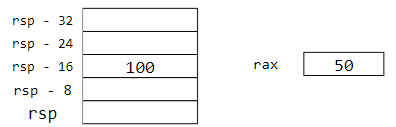
\includegraphics[scale=0.8]{assets/a3.png}} \\ 
        \hline 
        \code{add rax, [rsp - 16]} & \raisebox{-\totalheight}{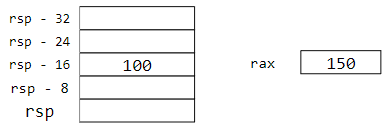
\includegraphics[scale=0.8]{assets/a4.png}} \\ 
        \hline 
        \code{mov [rsp - 16], rax} & \raisebox{-\totalheight}{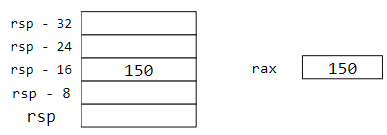
\includegraphics[scale=0.8]{assets/a5.png}} \\ 
        \hline 
        \code{mov rax, 2} & \raisebox{-\totalheight}{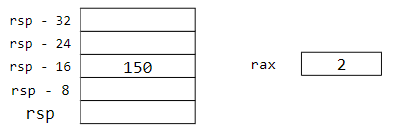
\includegraphics[scale=0.8]{assets/a6.png}} \\ 
        \hline 
        \code{add rax, [rsp - 16]} & \raisebox{-\totalheight}{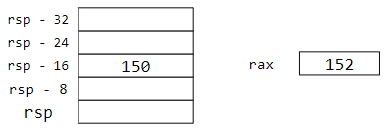
\includegraphics[scale=0.8]{assets/a7.png}} \\ 
        \hline 
    \end{tabular}
\end{center} 
\newpage
\section{Local Variables}
In this lecture, we want to add support for local variables through \code{let} expressions. 

\begin{mdframed}
    (Exercise.) Consider the following code.
    \begin{verbatim}
        (let (x 10)
            (let (y 10)
                (+ x y)))\end{verbatim}
    Using code discussed in the previous section, along with some intuition, what assembly do you think should be produced?

    \begin{mdframed}
    \end{mdframed}
    The assembly that could possibly be produced is as follows:
    \begin{center}
        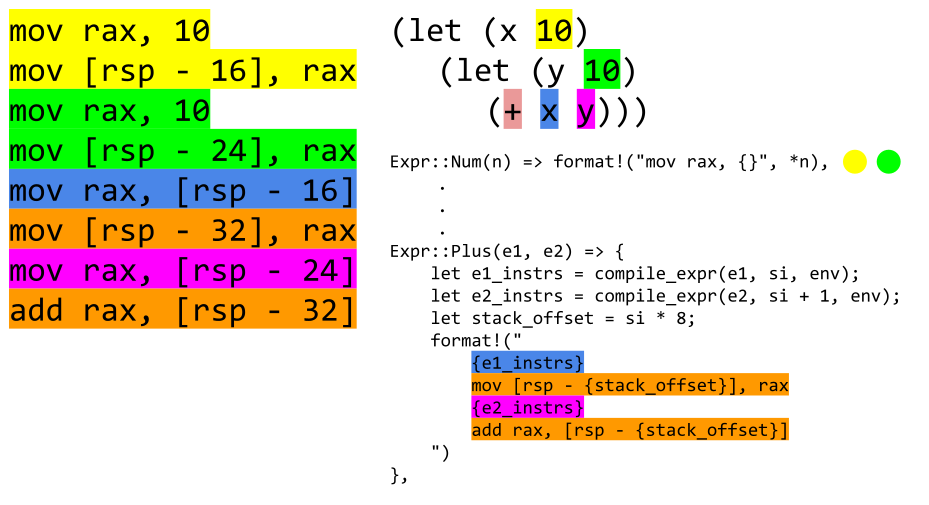
\includegraphics[scale=0.45]{assets/let_intro_asm.png}
    \end{center}
    
    At a high level, in terms of variable declaration, 
    \begin{itemize}
        \item We defined a local variable \code{x} with value \code{10}. So, it would make sense to store the value somewhere (e.g., at location \code{rsp - 16} in the stack). This corresponds to the first two lines of assembly, which are highlighted yellow.
        \item In the body of the first \code{let}-expression, we defined a local variable \code{y} with value \code{10}. So, again, it would make sense to store this value somewhere (e.g., at location \code{rsp - 24} in the stack, since we wouldn't want to overwrite the value at \code{rsp - 16}). This corresponds to the second two lines of assembly, highlighted orange. 
    \end{itemize}
    Next, we're performing the addition. Note that we're working with the expression \code{(+ x y)}. The assembly generated by the addition is found under the \code{Expr::Plus} branch.   
    \begin{itemize}
        \item It would make sense to put the value corresponding to \code{x} into our register where we're storing the answer, \code{rax}. Since the value corresponding to \code{x} is stored in the stack (at location \code{rsp - 16}), we need to \emph{move} the value over to \code{rax}. This corresponds to the fifth line in the assembly (highlighted blue). In this sense, we can assume that \code{e1\_instrs} returns just that line: \code{mov rax, [rsp - 16]}.
        \item Next, according to how we defined the instructions for addition, we need to move the value stored in \code{rax} to the stack memory, \code{[rsp - 32]}. This corresponds to the sixth line in the assembly (highlighted orange). Note that \code{32} is picked since we don't want to write this value to \code{rsp - 24} (this would overwrite \code{y}'s value.)
        \item Similarly, for variable \code{y}, we need to store its value into the register \code{rax}. Remember that \code{y}'s value is stored in the stack at location \code{rsp - 24}. So, we can move the value from this location to \code{rax}. This corresponds to the seventh line in the assembly (highlighted pink).
        \item Finally, from the last line in the \code{Expr::Plus} branch, we need to add the value stored at \code{rsp - 32} to \code{rax}. Recall that \code{[rsp - 32]} has \code{x}'s value (since we moved \code{x}'s value to \code{[rsp - 32]} from the previous two steps). This corresponds to the last line in the assembly (highlighted orange).
    \end{itemize}
    This gives us the desired result in \code{rax}.
\end{mdframed}
There are several things we want to consider here.
\begin{itemize}
    \item How do we modify the grammar and our code to account for these changes?
    \item How do we store the identifiers and their stack offsets? 
\end{itemize}

\subsection{Reviewing Assembly Instructions}
There are three assembly instructions you should know.
\begin{itemize}
    \item \code{mov <reg>, <value>}: moves \code{<value>} into \code{<reg>}. Note that \code{<value>} can either be a constant, another \code{reg}, or a memory location (e.g., \code{[rsp - X]}).
    \item \code{mov [<reg> + <offset>], <value>}: moves \code{<value>} into memory at address \code{<reg> + <offset>}. The \code{<value>} can be a constant or \code{reg}, but cannot be another memory location. 
    \item \code{add <reg>, <value>}: adds \code{<value>} to the value in \code{<reg>}, and stores the result in \code{<reg>}. The \code{<value>} can either be a constant, register, or memory location.  
\end{itemize}

\subsection{Grammar and AST}
Our expression now takes on two new forms:
\begin{itemize}
    \item A \code{let} expression, which takes a \emph{binding} consisting of an identifier and an associated expression, and additionally a corresponding body to be executed. 
    \item An identifier expression itself (this is how we refer to an identifier). 
\end{itemize}
Our grammar will look something like this: 
\begin{verbatim}
    (*
        expr := <number>
            | (add1 <expr>)
            | (sub1 <expr>)
            | (+ <expr> <expr>)
            | (let (<name> <expr>) <expr>)
            | <name>
    *)\end{verbatim}
The \code{Expr} \code{enum}, our AST representation, might look like 
\begin{verbatim}
    enum Expr {
        Num(i32),
        Add1(Box<Expr>),
        Sub1(Box<Expr>),
        Plus(Box<Expr>, Box<Expr>),
        Let(String, Box<Expr>, Box<Expr>),
        Id(String),
    }\end{verbatim} 
To reiterate, in \code{Let(String, Box<Expr>, Box<Expr>)}, 
\begin{itemize}
    \item The \code{String} and first \code{Box<Expr>} represents the \emph{binding}, where the \code{String} is the identifier and the first \code{Box<Expr>} is the expression. Here, we're associating the expression to the identifier. 
    \item The last \code{Box<Expr>} is the \emph{body} that follows the \code{let}-expression.
\end{itemize}

\subsection{Modifying the Parser}
We need to modify our parser to account for the two different expressions, the \code{let} expression and the identifier expression. 

\subsubsection{The \code{let}-Binding}
Remember that, in the s-expression, the \code{let}-binding will look like 
\begin{verbatim}
    (let (<name> <expr>) <expr>)
     [a]   [b]     [c]     [d]\end{verbatim}
Here, this corresponds to having a List of atoms and expressions. Namely, we have 
\begin{itemize}
    \item (a) an atom with a \code{String} value equal to \code{let} (this is how we know this is a \code{let}-binding),
    \item an \emph{expression}, represented as a \code{List}, with (b) an atom representing the identifier and (c) the expression to bind the identifier with.
    \item (d) the body of the \code{let}-statement, also an expression.
\end{itemize}

This gives us the following branch for \code{let}-bindings:
\begin{verbatim}
    [Sexp::Atom(S(op)), Sexp::List(binding), body] if op == "let" => {
        match &binding[..] {
            [Sexp::Atom(S(id)), expr] => {
                Expr::Let(id.to_owned(), Box::new(parse_expr(expr)),
                    Box::new(parse_expr(body)))
            }
            _ => panic!("parse error"),
        }
    }\end{verbatim}

\subsubsection{The Identifier Case}
Our identifier, like a number, is just by itself. For example, \code(+ 10 x) evaluates to $10 + x$, where $x$ is an atom. One thing to note is that identifiers are \emph{Strings}, just like how numbers are \emph{Integers}. So, this gives us the following branch for identifiers:
\begin{verbatim}
    Sexp::Atom(S(id)) => Expr::Id(id.to_owned()),\end{verbatim}


\subsubsection{Putting it Together}
Our parser now looks something like the below.
\begin{verbatim}
pub fn parse_expr(s: &Sexp) -> Expr {
    match s {
        Sexp::Atom(I(n)) => Expr::Num(i32::try_from(*n).unwrap()),
        Sexp::Atom(S(id)) => Expr::Id(id.to_owned()),
        Sexp::List(list) => match &list[..] {
            [Sexp::Atom(S(op)), e] if op == "add1" => 
                Expr::Add1(Box::new(parse_expr(e))),
            [Sexp::Atom(S(op)), e] if op == "sub1" => 
                Expr::Sub1(Box::new(parse_expr(e))),
            [Sexp::Atom(S(op)), e1, e2] if op == "+" => {
                Expr::Plus(Box::new(parse_expr(e1)), Box::new(parse_expr(e2)))
            }
            [Sexp::Atom(S(op)), Sexp::List(binding), body] if op == "let" => {
                match &binding[..] {
                    [Sexp::Atom(S(id)), expr] => {
                        Expr::Let(id.to_owned(), Box::new(parse_expr(expr)), 
                            Box::new(parse_expr(body)))
                    }
                    _ => panic!("parse error"),
                }
            }
            _ => panic!("parse error"),
        },
        _ => panic!("parse error"),
    }
}\end{verbatim}

\subsection{Modifying the Compilers}
There are some things we need to consider. 
\begin{itemize}
    \item We need to store all the identifiers and their stack offsets (where in the stack their values are stored in). For this, we can make use of a \code{HashMap<String, i32>}, which we'll call our \textbf{environment} (\code{env}). 
    \item Like with the parsing, we need to create two new branches for the \code{Let} case and the \code{Id} case.  
\end{itemize}
In this course, we'll make use of the \code{HashMap} implementation from the \code{im} crate (i.e., \code{im::HashMap}). The difference between this \code{HashMap} implementation and the one in the standard library is that \code{im::HashMap} will create a brand new \code{HashMap} object when you update the map, whereas the standard library version will update the original map. The reason why we're using \code{im::HashMap} is because we don't need to worry about removing the identifier from the map once we're done recursively calling the \code{compile\_expr} function.

\subsubsection{The Identifier Case}
The identifier is relatively straightforward. Notice how, in the exercise at the beginning of this section, whenever we refer to an identifier, we simply \emph{move} the value (stored in the stack) corresponding to the identifier to \code{rax}. 

\bigskip 

Remember that our map, \code{env}, has the identifier and its offset. So, we can \emph{get} the offset from the map and use that. 

\bigskip 

Therefore, the identifier case for the compiler looks like 
\begin{verbatim}
    Expr::Id(id) => format!("mov rax, [rsp - {}]", env.get(id.as_str()).unwrap()),\end{verbatim} 

\subsubsection{The \code{let}-Binding}
For the \code{Let} case, we have three associated values: the identifier, expression associated with the identifier, and the body associated with the binding itself. 

\bigskip 

At a high level, the idea is as follows:
\begin{itemize}
    \item First, we want to \emph{compile} the expression associated with the identifier. At the end, the value should be stored in \code{rax}. You can observe the other branches within the \code{compile\_expr} function (from the previous sections) to confirm this; in the branches, the last assembly instruction always involves moving or adding something \emph{to} \code{rax}. 
    \item Once we compiled the expression and have our result in \code{rax}, we need to do two things. 
    \begin{itemize}
        \item First, we need to store the result somewhere! We can make use of the current stack index to get the appropriate stack offset. Once we have this offset, we can \emph{move} the result in \code{rax} to that location in the stack.
        \item Next, we should probably store the identifier and where its value is stored in the stack (i.e., stack offset) in our environment \code{env}. So, we can just update the map to include this information. 
    \end{itemize}
    \item Now that we've done this, we can compile the body. Note that we want to increment the stack index by 1 when compiling the body -- otherwise, there's a real possibility that we'll overwrite the value stored in the stack (you know, the value corresponding to the identifier) with a different value.
\end{itemize}

This gives us the branch for the compiler,
\begin{verbatim}
    Expr::Let(id, ex, body) => {
        let ex_instr = compile_expr(ex, si, env);
        let new_env = env.update(id.to_owned(), si * 8);
        let body_instr = compile_expr(body, si + 1, &new_env);
        format!("
            {ex_instr}
            mov [rsp - {}], rax
            {body_instr}
        ", si * 8)
    }
\end{verbatim}

\subsubsection{Putting it Together}
Our compiler should now look something like the below.
\begin{verbatim}
fn compile_expr(e: &Expr, si: i32, env: &HashMap<String, i32>) -> String {
    match e {
        Expr::Num(n) => format!("mov rax, {}", *n),
        Expr::Add1(subexpr) => compile_expr(subexpr, si, env) + "\nadd rax, 1",
        Expr::Sub1(subexpr) => compile_expr(subexpr, si, env) + "\nsub rax, 1",
        Expr::Plus(e1, e2) => {
            let e1_instrs = compile_expr(e1, si, env);
            let e2_instrs = compile_expr(e2, si + 1, env);
            let stack_offset = si * 8;
            format!("
                {e1_instrs}
                mov [rsp - {stack_offset}], rax
                {e2_instrs}
                add rax, [rsp - {stack_offset}]
            ")
        },
        Expr::Let(id, ex, body) => {
            let ex_instr = compile_expr(ex, si, env);
            let new_env = env.update(id.to_owned(), si * 8);
            let body_instr = compile_expr(body, si + 1, &new_env);
            format!("
                {ex_instr}
                mov [rsp - {}], rax
                {body_instr}
            ", si * 8)
        }
        Expr::Id(id) => format!("mov rax, [rsp - {}]", env.get(id.as_str()).unwrap()),
    }
}
\end{verbatim}
\newpage
\section{Introduction to \code{if}-Expressions}
In this section, we'll discuss how to implement \code{if}-expressions. Our concrete syntax for this extension will look like 
\begin{verbatim}
(*
    expr :=
        | <number>
        | true                              // New!
        | false                             // New!
        | <name>
        | (add1 <expr>)
        | (sub1 <expr>)
        | (+ <expr> <expr>)
        | (let (<name> <expr>) <expr>)
        | (if <expr> <expr> <expr>)         // New!
        | ... 
*)\end{verbatim}

\subsection{Structure of \code{if}-Expressions}
An \code{if}-expression looks like 
\begin{verbatim}
    (if <expr> <expr> <expr>)\end{verbatim}

\begin{itemize}
    \item Here, the first \code{<expr>} represents the condition expression; this determines which of the subsequent expressions should be executed. 
    \item The second \code{<expr>} represents the ``then'' expression; this expression should be executed if the condition expression resolves to \code{true}.
    \item The third and last \code{<expr>} represents the ``else'' expression; this expression should be executed if the condition expression resolves to \code{false}.
\end{itemize}
Before we talk more about how \code{if}-expressions should be evaluated, we need to figure out how \code{if}-expressions should work in the first place in terms of what is allowed and what isn't. 

\subsection{Boolean Values}
Let's begin by figuring out what some sample programs should resolve to.
\begin{mdframed}
    (Exercise.) What should the following programs evaluate to? 
    \begin{enumerate}[a.]
        \item \begin{verbatim}
(let (x 5)
    (if (= x 10) (+ x 2) x))\end{verbatim}

        \begin{mdframed}
            This should evaluate to \code{5}. We first defined $x = 5$ and then used that in our \code{if}-expression to see if $x = 10$; since it doesn't, we just return \code{x}, which is 5.  
        \end{mdframed}


        \item \begin{verbatim}
(if 5 true false)\end{verbatim}

        \begin{mdframed}
            There are several reasonable answers we can consider here. 
            \begin{itemize}
                \item \code{true}: since \code{5} is a truthy value (i.e., evaluates as a true expression), it would make sense for this program to return \code{true}.
                \item \code{false}: since \code{5} isn't a boolean expression, we could just have the program return \code{false}.
                \item an error: since \code{5} isn't a boolean expression, we can throw an error telling the user that this isn't an boolean expression. 
            \end{itemize}
            In our class, we'll say \code{true}. In other words, we're allowing truthy and falsy values.
        \end{mdframed}


        \item \begin{verbatim}
(+ 7 true)\end{verbatim}

        \begin{mdframed}
            There are two answers we can have for this. 
            \begin{itemize}
                \item \code{8}: if \code{true} implicitly resolves to \code{1}, then this is just $7 + 1 = 8$.
                \item an error: since \code{7} and \code{true} are different types, it wouldn't make sense to add them. 
            \end{itemize}
            In our class, we'll say that this expression should throw an error at compile-time.
        \end{mdframed}

        \item \begin{verbatim}
(= true 1)\end{verbatim}

        \begin{mdframed}
            There are two answers we can have for this. 
            \begin{itemize}
                \item \code{true}: for the same reason as above.
                \item an error: for the same reason as above. 
            \end{itemize}
            In our class, we'll say that this expression should throw an error at compile-time.
        \end{mdframed}
    \end{enumerate}
\end{mdframed}
Based on our discussion above, in this class, 
\begin{itemize}
    \item We'll allow truthy and falsy values to be resolved to boolean types (\code{true} and \code{false}, respectively) when used as conditions in \code{if}-expressions.
    \item We won't allow the mixing of types when doing comparison (e.g., \code{=}, \code{<}, etc.) or arithmetic (e.g., \code{+}, \code{-}) operations. These should throw an error during runtime\footnote{In our class, we won't be working on a type checker. However, if we did work on a type checker, then we could make mixing of types when doing these operations a compile-time (parse) error.}.
\end{itemize}

\subsection{Boolean Representation}
With the above discussion in mind, how should we best represent boolean values in assembly?

\begin{mdframed}
    (Exercise.) \emph{Intuitively} (i.e., using our knowledge from previous sections), what should be in \code{RAX} after these are done evaluating? 

    \begin{enumerate}[a.]
        \item \code{1}
        \begin{mdframed}
            Trivially, we just move \code{1} into \code{RAX}.
        \end{mdframed}

        \item \code{5}
        \begin{mdframed}
            Trivially, we just move \code{5} into \code{RAX}.
        \end{mdframed}

        \item \code{-3}
        \begin{mdframed}
            Trivially, we just move \code{-3} into \code{RAX}.
        \end{mdframed}

        \item \code{true}
        \begin{mdframed}
            There's not exactly a way to directly represent \code{true} in assembly, so the best we can do is a truthy value. For now, let's just move \code{1} into \code{RAX}.
        \end{mdframed}

        \item \code{false}
        \begin{mdframed}
            Same idea as before: the best we can do is a falsy value. For now, let's just move \code{0} into \code{RAX}.
        \end{mdframed}

        \item \code{(= 3 5)}
        \begin{mdframed}
            Since $3 = 5$ is false, we can just put \code{0} into \code{RAX}.
        \end{mdframed}

        \item \code{(+ 4 7)}
        \begin{mdframed}
            Trivially, we just move the result of $4 + 7$, or \code{11}, into \code{RAX}.
        \end{mdframed}
    \end{enumerate}
\end{mdframed}
Remember that we didn't want the mixing of types when doing any comparison or arithmetic operations, e.g., \code{(+ 5 true)} should throw an error. However, with our answers above, how do we know that the \code{1} in \code{RAX} isn't actually a \code{true} value? 

\subsection{A New Representation of Numbers: Tagging}
We will now represent numbers as \textbf{64-bits} instead of 32-bits like in previous sections. With this in mind, this is 64 bits:
\begin{verbatim}
    0000 0000 0000 0000 0000 0000 0000 0000 0000 0000 0000 0000 0000 0000 0000 0000\end{verbatim}
The number 5 can be represented like so: 
\begin{verbatim}
    0000 0000 0000 0000 0000 0000 0000 0000 0000 0000 0000 0000 0000 0000 0000 0101\end{verbatim}

Let's suppose we \emph{shift} 5 one to the left to get the number 10: 
\begin{verbatim}
    0000 0000 0000 0000 0000 0000 0000 0000 0000 0000 0000 0000 0000 0000 0000 1010\end{verbatim}

If we're okay with 63-bit numbers, we can use the \textbf{least significant bit} (i.e., the right-most bit) as a \textbf{tag}. This tag tells us if the value is a number or a boolean value. In this class, 
\begin{itemize}
    \item Numbers will have a least significant bit of \code{0}.
    \item Booleans will have a least significant bit of \code{1}. 
\end{itemize}
For example, we can represent the number \code{13} as 
\begin{verbatim}
    0000 0000 0000 0000 0000 0000 0000 0000 0000 0000 0000 0000 0000 0000 0001 1010\end{verbatim}
We can represent the boolean \code{false} as 
\begin{verbatim}
    0000 0000 0000 0000 0000 0000 0000 0000 0000 0000 0000 0000 0000 0000 0000 0001\end{verbatim}
We can represent the boolean \code{true} as 
\begin{verbatim}
    0000 0000 0000 0000 0000 0000 0000 0000 0000 0000 0000 0000 0000 0000 0000 0011\end{verbatim}
We can represent the number \code{0} as 
\begin{verbatim}
    0000 0000 0000 0000 0000 0000 0000 0000 0000 0000 0000 0000 0000 0000 0000 0000\end{verbatim}
    
\subsection{Consequences of Tagging}
Because we effectively have to shift everything one to the left to introduce tagging, we need to think about a few things.
\begin{itemize}
    \item \underline{\textbf{Addition}}
    \begin{itemize}
        \item When we are performing any binary (or unary) operations, we need to check if the least significant bit is correct for the given input. For example, when we are doing addition, we should check if the least significant bit of both inputs are \code{0} (implying that both are numbers). If any one of them isn't, then we should throw an error.
        \item Otherwise, addition is pretty straightforward. Assuming we have two numbers, adding two numbers should not change since the addition of both least significant bits will be 0 (since $0 + 0 = 0$). In other words, something like \code{(+ 3 5)} will generate the assembly 
        \begin{verbatim}
    mov rax, 6              ; 3 / 11 (decimal / binary)  
                            ; -> 6 /   110 (decimal / binary) accounting for tag
    mov [rsp - 16], rax 
    mov rax, 10             ; 5 / 101 (decimal / binary) 
                            ; -> 10 / 1010 (decimal / binary) accounting for tag 
    add rax, [rsp - 16]     ; 6 + 10 -> 10000 (with tagging)\end{verbatim}
        Notice how \code{10000} in binary is \code{16} in decimal. However, if we shift this answer by one to the \emph{right}, we get \code{8}, the answer to $3 + 5$.
    \end{itemize}
    \item \underline{\textbf{Multiplication}}
    \begin{itemize}
        \item Multiplication is similar to addition, except we want to make sure we shift one of the two inputs by 1 to the right before we perform the actual multiplication. So, \code{(* 3 5)} should produce the assembly
        \begin{verbatim}
            mov rax, 6              ; 3 ->  1100 accounting for tag
            mov [rsp - 16], rax 
            mov rax, 10             ; 10 -> 1010 accounting for tag
            sar rax, 1              ; 5  ->  101 (remove tagging)
            imul rax, [rsp - 16]    ; 6 * 5 -> 11110000\end{verbatim}
        \code{11110} in binary is \code{30} in decimal. Shifting this by 1 to the right gives us the desired answer of \code{15}. The reason why we choose to shift one of the two values to the right by 1 is so we can avoid potential overflow errors.
    \end{itemize}

    \item \underline{\textbf{Errors}}
    \begin{itemize}
        \item If we get an error (e.g., a type mismatch error), then from our assembly code, we want to call a \emph{Rust} function that handles the error. 
        \item For example, we might have something like 
        \begin{verbatim}
            and rax, 1 
            cmp rax, 1      ; if we get a boolean value instead of number
            je error_label  ; jump to the error_label error 
                            ; otherwise, fall through label
            ...
        error_label: 
            call rust_error\end{verbatim}
        with corresponding Rust code 
        \begin{verbatim}
            fn error() {
                panic!("error");
            }\end{verbatim}
    \end{itemize}
\end{itemize}


\subsection{Assembly Review}
There are some new assembly commands to know.
\begin{itemize}
    \item \code{cmp <reg>, <val>}: computes \code{<reg> - <val>} and sets the appropriate condition codes\footnote{The only ones that matter to us are Overflow, Sign, and Zero}. This does not modify \code{<reg>}.
    \item \code{<label>:  }: Sets this line as a label for jumping to later. 
    \item \code{and <reg>, <value>}: Performs bitwise AND on \code{<reg>} and \code{<value>}. 
    \item \code{jmp <label>}: Unconditionally jumps to \code{<label>}.
    \item \code{jne <label>}: Jumps to \code{<label>} if Zero is not set (last \code{cmp}ed values not equal).
    \item \code{je <label>}: Jumps to \code{<label>} if Zero is set (last \code{cmp}ed values equal).
    \item \code{jge <label>}: Jumps to \code{<label>} if Overflow is the same as Sign (corresponds to \code{>=} for last \code{cmp}).
    \item \code{jle <label>}: Jumps to \code{<label>} if Zero is set or Overflow is not equal to Sign (corresponds to \code{<=} for last \code{cmp}).
    \item \code{shl <reg>}: Shifts \code{<reg>} to the left by 1, filling in least-significant bit with zero.
    \item \code{sar <reg>}: Shifts \code{<reg>} to the right by 1, filling in most-significant bit to preserve sign
    \item \code{shr <reg>}: Shifts \code{<reg>} to the right by 1, filling in most-significant bit with zero.
\end{itemize}

\subsection{Modifying the Runtime}
In our class, we had a \code{runtime.rs} file which was responsible for calling our assembly code and printing out the result; this looks something like:
\begin{verbatim}
    #[link(name = "our_code")]
    extern "C" {
        #[link_name = "\x01our_code_starts_here"]
        fn our_code_starts_here() -> i64;
    }
    
    fn main() {
        let i: i64 = unsafe { our_code_starts_here() };
        println!("{i}");
    }\end{verbatim}
One thing to consider here is that, with our new tagging system, we have two problems
\begin{itemize}
    \item The code above won't print out boolean values properly (it'll either print out \code{3} or \code{1}, not \code{true} or \code{false} like we would hope).
    \item It also won't print out the numbers correctly. Remember that the integers have been shifted one bit to the left, and this code doesn't account for that when printing the result. So, if the code is supposed to print \code{5}, then this would actually print \code{10}. 
\end{itemize}
The solution is to modify this file so that it can correctly interpret the resulting value that the assembly code produces. We might have something like the below.
\begin{verbatim}
    fn main() {
        let i: i64 = unsafe { our_code_starts_here() };
        // If we have an integer (remember that, for numbers, the LSB should be 0)
        if i & 1 == 0 {
            println!("{}", i >> 1);
            return;
        }

        // Otherwise, i & 1 -> 1, so we should have a boolean value. Let b 
        // be either 0 or 1 (if we have a valid boolean).
        let b = i >> 1;
        // If b is 0 or 1, then we have a boolean value.
        if b == 0 || b == 1 {
            println!("{}", b == 1);
        } else {
            println!("unknown value: {i}");
        }
    }\end{verbatim}

\subsection{The Abstract Syntax}
Recall that an \code{if}-expression looks something like 
\begin{verbatim}
    (if <expr> <expr> <expr>)\end{verbatim}
where 
\begin{itemize}
    \item the first \code{<expr>} represents the condition expression; this determines which of the subsequent expressions should be executed. 
    \item the second \code{<expr>} represents the ``then'' expression; this expression should be executed if the condition expression resolves to \code{true}.
    \item the third and last \code{<expr>} represents the ``else'' expression; this expression should be executed if the condition expression resolves to \code{false}.
\end{itemize}
As defined in the grammar, we also need to be able to support boolean values (\code{true} and \code{false}). This is trivially just \code{True} and \code{False} in the abstract syntax. So, the abstract syntax will look like 
\begin{verbatim}
    enum Expr {
        Num(i32),
        True,                                   // New!
        False,                                  // New!
        Add1(Box<Expr>),
        Plus(Box<Expr>, Box<Expr>),
        Let(String, Box<Expr>, Box<Expr>),
        Id(String),
        Eq(Box<Expr>, Box<Expr>),               // New!
        If(Box<Expr>, Box<Expr>, Box<Expr>)     // New!
    }\end{verbatim}

\subsection{Extending the Parser}
Because our \code{if}-expression is basically a list of four expressions, we just need to match that particular pattern. So, parsing \code{if}-expressions should be straightforward. 
\begin{verbatim}
    match s {
        ...
        Sexp::List(list) => match &list[..] {
            [Sexp::Atom(S(keyword)), cond, thn, els] if keyword == "if" => Expr::If(
                Box::new(parse_expr(cond)),
                Box::new(parse_expr(thn)),
                Box::new(parse_expr(els)),
            )
            ...    
        }
    }\end{verbatim}
So, how do we represent boolean types? One way is by looking at the identifier: if the identifier happens to be \code{true} or \code{false}, we can assume that this is a \code{boolean} type. Otherwise, we can assume that we just have a regular identifier.
\begin{verbatim}
    match s {
        Sexp::Atom(S(id)) => {
            if id == "true" {
                Expr::True
            } else if id == "false" {
                Expr::False
            } else {
                Expr::Id(id.to_owned())
            }
        }
        ...
    }\end{verbatim}
Finally, parsing the equality operator (e.g., \code{(= 10 5)}) is the same as with parsing the plus operator.

\subsection{Implementing the Compiler}
Before we start, one adjustment we need to make to account for the tagging system that we've discussed is to shift integers one bit to the left. That is, when we have an integer, we need to shift it one bit to the left so the least significant bit can be used as the tag bit.
\begin{verbatim}
    match e {
        Expr::Num(n) => format!("mov rax, {}", *n << 1),
        ... 
    }\end{verbatim}
Now, let's think about \code{if}-expressions. \code{if}-expressions imply that only a subset of code will be executed. For example, if we have an \code{if}-statement and the condition resolves to \code{false}, the code inside the \code{if}-statement will not be executed. In assembly, we can represent this behavior using \textbf{branches}. Roughly speaking, the assembly will look like
\begin{verbatim}
        cmp value, 3        ; if value == true {
        jne else_block      ;       // your code
        // code here        ;       // here 
        jmp done_block      ; 
    else_block:             ; } else {
        // code here        ;       // your code here
    done_block:             ; }
\end{verbatim}
What's going on?  
\begin{center}
    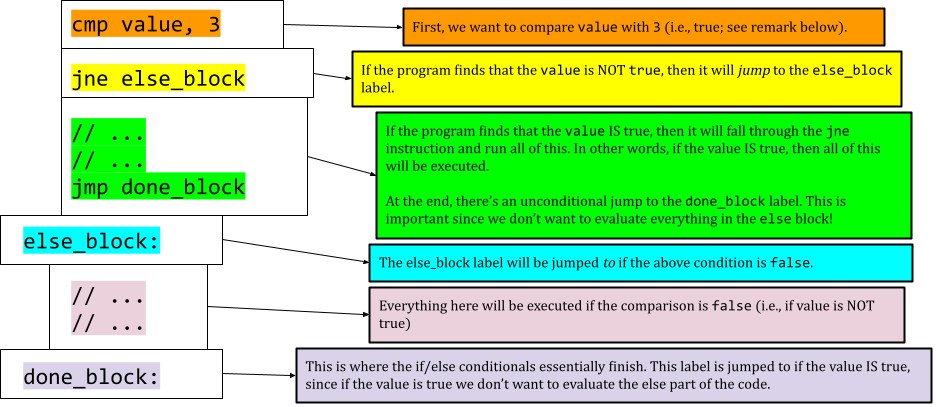
\includegraphics[scale=0.5]{assets/asm_if.png}
\end{center}
\textbf{Remark:} \code{3} is represented as \code{true} (the binary representation of \code{3} is \code{11}; notice how the tag bit is \code{1}).

\subsubsection{Duplicate Labels}

All \code{if}-expressions will follow the same pattern\footnote{Maybe not the exact pattern, but the same behavior}. However, if we just use this same exact template, we'll end up with multiple duplicate label declarations. In other words, we might end up with something like 
\begin{verbatim}
    cmp value 3
    jne else_block 
    // ... 
    jmp done_block 
else_block:
    // ... 
done_block:
    // ...
    cmp value 3
    jne else_block 
    // ... 
    jmp done_block 
else_block:
    // ... 
done_block:\end{verbatim}
This code would fail to run since there are, for example, duplicate \code{done\_block} label declarations. So, we need to create a unique label whenever we do declare a label. Let's declare a function that does just this: 
\begin{verbatim}
    fn new_label(l: &mut i32, s: &str) -> String {
        let current = *l;
        *l += 1;
        format!("{s}_{current}")
    }\end{verbatim}
At a high level, \code{new\_label} takes in a mutable reference to an integer and a string, and creates a label using those inputs. The integer is incremented -- this is important since this guarantees that every label created from this function will be unique.

\subsubsection{The Equals Comparison Operator}
How do we check if two expressions are equal? The process is relatively similar to adding two expressions. The only difference is at the end, when instead of actually \emph{adding} the values, we put either 3 (\code{true}) or 1 (\code{false}) into \code{rax}.

\bigskip 

The way we do this (putting either \code{3} or \code{1} into \code{rax}) is literally just another \code{if}-statement! At a high level, this might look like: 
\begin{verbatim}
    if rax == [rsp - stack_offset] {
        rax = 3
    } else {
        rax = 1
    }\end{verbatim}
So, compilation might look something like this: 
\begin{verbatim}
    match e {
        Expr::Eq(a, b) => {
            let a_instr = compile_expr(a, si, env, counter);
            let b_instr = compile_expr(b, si + 1, env, counter);
            let else_label = new_label(counter, "ifelse");
            let end_label = new_label(counter, "ifend");
            let stack_offset = si * 8;

            format!("
            {a_instr}
            mov [rsp - {stack_offset}], rax
            {b_instr}
            cmp rax, [rsp - {stack_offset}]
            jne {else_label}
              mov rax, 3
              jmp {end_label}
            {else_label}:
              mov rax, 1
            {end_label}:
            ")
        }
        ...
    }\end{verbatim}

\subsubsection{\code{if}-Expressions}
With everything in mind, our final implementation of \code{if}-expressions will look something like the below.
\begin{verbatim}
    match e {
        Expr::If(cond, thn, els) => {
            let end_label = new_label(counter, "ifend");
            let else_label = new_label(counter, "ifelse");
            let cond_instrs = compile_expr(cond, si, env, counter);
            let thn_instrs = compile_expr(thn, si, env, counter);
            let els_instrs = compile_expr(els, si, env, counter);
            format!(
                "
               {cond_instrs}
               cmp rax, 3
               jne {else_label}
                 {thn_instrs}
                 jmp {end_label}
               {else_label}:
                 {els_instrs}
               {end_label}:"
            )
        }
        ... 
    }\end{verbatim}
At a high level, 
\begin{itemize}
    \item First, we should evaluate the conditional part of the \code{if}-statement. We should\footnote{We'll talk more about type validation later.} end up with a boolean value in \code{rax}. 
    \item With the boolean value in \code{rax}, we can determine which code (either the ``then'' or ``else'' blocks) to run. 
\end{itemize}
\newpage
\section{An Overview of Loops, Set, Break, Input, Blocks, and Errors}
In this section, we'll go over a high-level overview of some additional features. 

\subsection{Loops \& Break}
Loop and break expressions are relatively simple; they look something like 
\begin{verbatim}
    (loop <expr>)
    (break <expr>)\end{verbatim}
At its core, a \code{loop} will repeat an expression over and over again until it encounters a \code{break}, in which case the loop terminates.

\subsubsection{Assembly Representation} 
The assembly representation of loops is straightforward:
\begin{verbatim}
    loop: 
                    ; body of loop 
        jmp loop 
    done:\end{verbatim}
Here, we defined two labels: 
\begin{itemize}
    \item \code{loop}, indicating the beginning of the loop. 
    \item \code{done}, indicating the end of the loop (where we should ``break'' out).
\end{itemize}
The idea is that, as long as we aren't breaking out, we will unconditionally jump back to \code{loop}. If we do want to incorporate a \code{break} statement, we can add a jump to that label.

\subsubsection{Labeling}
As is the case with \code{if}-statements, we can have many loops! So, we need to create a unique label for each loop. We can use the \code{new\_label} function from the last section to do this for us. 

\subsubsection{Implementing Break}
To implement \code{break}, the idea is for the compiler to include an additional argument. We can call this argument \code{loop\_label}, which will be an \code{Option<String>} (recall that an \code{Option<T>} will either be a \code{Some(T)} or \code{None}, indicating some or no value, respectively).

\bigskip 

Before we compile the expression associated with the loop, we need to create a unique label. Once we create this label, we can compile the expression, passing that label as our argument for \code{loop\_label}. Because of the recursive nature of the compile function, if we end up inside another loop, compiling its associated expression will result in another label for \emph{that} function call, but not for the current function call. In that sense, we don't need to worry about the possibility of overwriting the break labels.

\subsection{Set}
Set is relatively straightforward: it's analogous to reassignment in most other programming languages. Its syntax looks like 
\begin{verbatim}
    (set! <name> <expr>)\end{verbatim}
Here, we're assigning the result of evaluating \code{<expr>} to the identifier, \code{<name>}. If the identifier doesn't exist, an error should be thrown. 

\subsection{Blocks}
Blocks are just a way of writing more than one statement for an expression. Syntactically, they look like 
\begin{verbatim}
    (block <expr>+)\end{verbatim}
In other words, it takes one or more expressions, and then runs each expression in the order that they appear.

\begin{center}
    \begin{tabular}{p{3in}|p{3in}}
        Rust & Our Language \\ 
        \hline 
        \begin{verbatim}
if x > 10 {
    x = x + y + z;
    y = x - z;
    z = z + 5;
} else {
    x += 10;
}\end{verbatim} 
            & \begin{verbatim}
(if (> x 10) 
    (block 
        (set! x (+ x (+ y z)))
        (set! y (- x z))
        (set! z (+ z 5))
    ) 
    (set! x (+ x 10)))\end{verbatim}
    \end{tabular}
\end{center}

\subsection{Handling Inputs}
Our programming language is now expected to take a single input, which can either be a number or boolean value. Syntactically, the command is just 
\begin{verbatim}
    input \end{verbatim}
In order to handle any input, we need to think about the runtime and, more importantly, the role that \code{start.rs} plays (recall that \code{start.rs} is how we call into our assembly code.)
\begin{verbatim}
    fn parse_input(input: &str) -> i64 {
        if input == "true" {
            0b11
        } else if input == "false" {
            0b01
        } else if let Ok(val) = input.parse::<i64>() {
            (val << 1) as u64
        } else {
            panic!("unsupported input: `{}`", input);
        }
    }

    fn main() {
        let args: Vec<String> = env::args().collect();
        // This is our single input, which by default will be 
        // "false" if none are provided
        let input = if args.len() == 2 { &args[1] } else { "false" };
        // Call our assembly code with the given input.
        let i: i64 = unsafe { our_code_starts_here(parse_input(&input)) };
        // Finally, determine what was returned to us.
        if i & 1 == 0 {
            // Number
            println!("{}", i >> 1);
        } else {
            // Boolean
            println!("{}", i >> 1 == 1);
        }
    }\end{verbatim}
Note that our input will be in the register \code{rdi}. So, we can modify the compiler to simply move \code{rdi} into \code{rax} before using it. 
\begin{verbatim}
    match e {
        ... 
        Expr::Id(s) if s == "input" => "mov rax, rdi"
    }\end{verbatim}
That's it!

\subsection{Errors}
Recall that, in the previous sections, we didn't want things like \code{(+ true 1)} to work. This should cause a \emph{runtime error}. So, how do we invoke a runtime error from our assembly code? 
\begin{itemize}
    \item First, we want to create a function in Rust that our assembly code will call. 
    \begin{verbatim}
    #[export_name = "\x01snek_error"]
    pub extern "C" fn snek_error(errcode: i64) {
        eprintln!("error code {errcode} received.");
        std::process::exit(1);
    }\end{verbatim}
    
    \item Next, in our assembly header, we want to define this function as an external function. 
    \begin{verbatim}
        section .text 
        global our_code_starts_here 
        extern snek_error               ; right here!\end{verbatim}

    \item From there, we can define a \code{throw\_error} label which will handle calling the Rust code. It will look like 
    \begin{verbatim}
        throw_error: 
            mov rdi, 7          ; rdi is the register representing the first arg 
                                ; 7 is some error code we made up 
            push rsp    
            call snek_error     ; calls the snek_error rust function 
            ret \end{verbatim}
    We'll worry about the \code{push} and \code{pop} instruction later. 
\end{itemize}
\newpage
\section{Introduction to Calling Conventions: Print}
In the previous section, we discussed throwing errors and how we can call an external (Rust) function from our generated assembly code. Note that the error case is interesting in the sense that it always terminated the program, so we didn't have to worry about coming back to our generated code.

\bigskip 

Suppose we want to introduce a \code{print} expression, which takes an expression and then prints the result out. Like the error handling, the \code{print} expression will call an external Rust function. However, unlike the error handling, we expect the \code{print} expression to come back to the generated assembly code \emph{after} calling the external function.

\bigskip 

Syntactically, \code{print} looks like 
\begin{verbatim}
    <expr> := ... | input | (print <expr>)\end{verbatim}

\subsection{Modifying \code{start.rs}}
Once again, as we need to define a function in Rust to handle printing so our generated assembly code can use it, we need to modify \code{start.rs} to include this information. Let's define the following function to handle printing: 
\begin{verbatim}
    #[no_mangle]
    #[export_name = "\01snek_print"]
    fn snek_print(val : i64) -> i64 {
        if val == 3 { println!("true"); }
        else if val == 1 { println!("false"); }
        else if val % 2 == 0 { println!("{}", val >> 1); }
        else {
            println!("Unknown value: {}", val);
        }
        return val;
    }\end{verbatim}
Note that 
\begin{itemize}
    \item \code{3} is our representation of \code{true} (\code{3} is \code{0b11} in binary.)
    \item \code{1} is our representation of \code{false} (\code{1} is \code{0b01} in binary.)
\end{itemize}

\subsection{Calling Convention Idea}
At a high level, when calling a function, we need to do the following: 
\begin{enumerate}
    \item ``Remember where'' we left off (i.e., recovering the stack).
    \item Pass in the appropriate arguments. 
    \item Call the \code{snek\_print} function.
\end{enumerate}
Regarding ``remember where'' we left off: remember that our compiler function has a parameter which represents the stack index. This stack index tells us how ``deep'' we are in the expressions that needed temporary storage/variables. So, whatever stack index we have, we need to set up the call so that it's above the stack index; after the call is done, we need to go back to where the stack index was originally.

\subsection{Implementing \code{print}}
Let's now attempt to implement \code{print} into our compiler.

\subsubsection{Attempt 1}
Our initial implementation of \code{print} might look like 
\begin{verbatim}
match e {
    ... 
    | Expr::Id(s) if s == "input" => "mov rax, rdi".to_string(),
    | Expr::Print(val) => {
        let offset = si * 8; 
        let v_is = compile_expr(val, si, env, l);
        format!("
            {v_is}
            sub rsp, {offset}
            mov rdi, rax 
            call snek_print
            add rdi, {offset}
        ")
    }
}\end{verbatim}
In terms of what's going on, what \verb|sub rsp, {offset}| is doing is moving \code{rsp}, the stack pointer, so that it's pointing \emph{above} where all the local variables and temporaries are.  
\begin{center}
    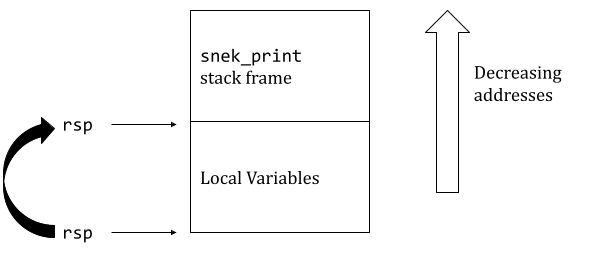
\includegraphics[scale=0.5]{assets/rsp_offset_subtract.png}
\end{center}
So, the stack frame for the \code{snek\_print} is where all the work for this function will happen. So, being its own function, it will rely on \code{rsp} being ``kind of'' like at bottom of its stack frame, since it gets its own local variable space whatnot. 

\begin{mdframed}
    (Exercise.) Consider the following code: 
    \begin{verbatim}
(block 
    (print 37)
    (print input)
)\end{verbatim}
    Using our implementation above, what would be printed if \code{input} was \code{true}? 

    \begin{mdframed}
        This would print \code{37} twice. To see why, let's consider the generated assembly.
        \begin{verbatim}
            mov rax, 74
            sub rsp, 16 
            mov rdi, rax 
            call snek_print 
            add rsp, 16 
            mov rax, rdi 
            ... \end{verbatim}
        The issue is in the third line, \code{mov rdi, rax}. We're overwriting \code{rdi}, which contains the result of \code{input}, with a different value! More specifically, we used \code{rdi} to pass in the argument for \code{print}, but this means we lose the result of \code{rdi} when we passed in the argument.
    \end{mdframed}
\end{mdframed}
So, we just need to remember to store data from registers somewhere else before we do the call. One thing we can do is store \code{rdi} somewhere on the stack before we make the function call. To do this, we can make use of \code{push} and \code{pop}. In fact, \code{rdi} is an example of a \textbf{caller-saved register}; that is, before we make a function call, we should save this register if we want to restore it afterwards. 

% https://stackoverflow.com/questions/9268586/what-are-callee-and-caller-saved-registers 

\subsubsection{Attempt 2}
With what we just mentioned in mind, we have 
\begin{verbatim}
    match e {
        ... 
        | Expr::Id(s) if s == "input" => "mov rax, rdi".to_string(),
        | Expr::Print(val) => {
            let offset = si * 8; 
            let v_is = compile_expr(val, si, env, l);
            format!("
                {v_is}
                sub rsp, {offset}
                push rdi            ; added this line 
                mov rdi, rax 
                call snek_print
                pop rdi             ; added this line 
                add rdi, {offset}
            ")
        }
    }\end{verbatim}
\textbf{Remark:} Remember that we want \code{rsp} to point to the spot where the pop is going to be, which is why we call \code{pop rdi} immediately after the \code{call} call. 

\bigskip 

Note that 
\begin{itemize}
    \item \code{push} pushes a value (register, immediate, etc.) to the stack. \code{push} will subtract 1 from \code{rsp}. 
    \item \code{pop} pops whatever is on top of the stack into a register. \code{pop} will add 1 to \code{rsp}. 
\end{itemize}
\begin{mdframed}[nobreak=true]
    (Example.) For example, 
    \begin{verbatim}
        push 17 
        push 23 
        pop rax 
        pop rcx \end{verbatim}
    will put \code{23} into \code{rax}, and \code{17} into \code{rcx}.
\end{mdframed}
So, in terms of what the generated assembly would do, it would 
\begin{itemize}
    \item Push \code{rsp} into the stack. 
    \item Then, move \code{rax} into \code{rsp}.
    \item Then, call the \code{snek\_print} function. 
    \item Then, put the most recently added value from stack (i.e, the old value of \code{rsp}) to the register \code{rsp}.
\end{itemize}
It just so happens that, in our example here, we only really care about \code{rdi}. But, if we have other registers that we care about (e.g., we use them a lot or need to save them between expressions), we need to save them. 

\subsection{Alignment Issues}
To summarize some of the things we've said about the x86\_64 calling convention\footnote{These are calling conventions specific to x86\_64, and is the reason why we had to do this when calling \code{snek\_print}. However, when we define our own functions in our own language, we can use whatever calling convention we want (including making one up) as long as it's consistent. }:
\begin{itemize}
    \item Arguments go into \code{rdi}, and then 6 other registers, and then the stack.
    \item \code{[rsp]} (i.e., the value stored at location \code{rsp}) should be the return pointer.
    \item 16-byte alignment constraint: $\code{rsp} \Mod{16} = 0$.
\end{itemize}
So, in our generated assembly, the third point may cause some problems with the stack pointer. One way we can resolve this is to check what $\code{stack\_offset} \Mod{16}$ is, or equivalently $\code{stack\_index} \Mod{2}$ is. For the latter, if we have an odd number, we can add 1 to the stack index so we have an even stack index.
\newpage
\section{Calling Conventions}
In this section, we'll talk more about calling conventions. 

\subsection{Argument Conventions in x86\_64}
Consider the following code (assuming that only this part of the code has changed.)
\begin{verbatim}
    #[link(name = "our_code")]
    extern "C" {
    #[link_name = "\x01our_code_starts_here"]
        fn our_code_starts_here(input : i64, p1 : i64, p2 : i64, ..., p8 : i64) -> i64;
    }

    fn main() {
        let args: Vec<String> = env::args().collect();
        let input = parse_arg(&args);
        let i : i64 = unsafe { 
            our_code_starts_here(input, 9, 10, 11, 12, 13, 14, 15, 16) 
        };
        snek_print(i);
    }\end{verbatim}
Here, we added 8 parameters to the \code{our\_code\_starts\_here} function so we can see how the arguments are represented in memory. Using \code{rust-lldb}, we can debug this code and, more importantly, see the memory layout of our program.
\begin{center}
    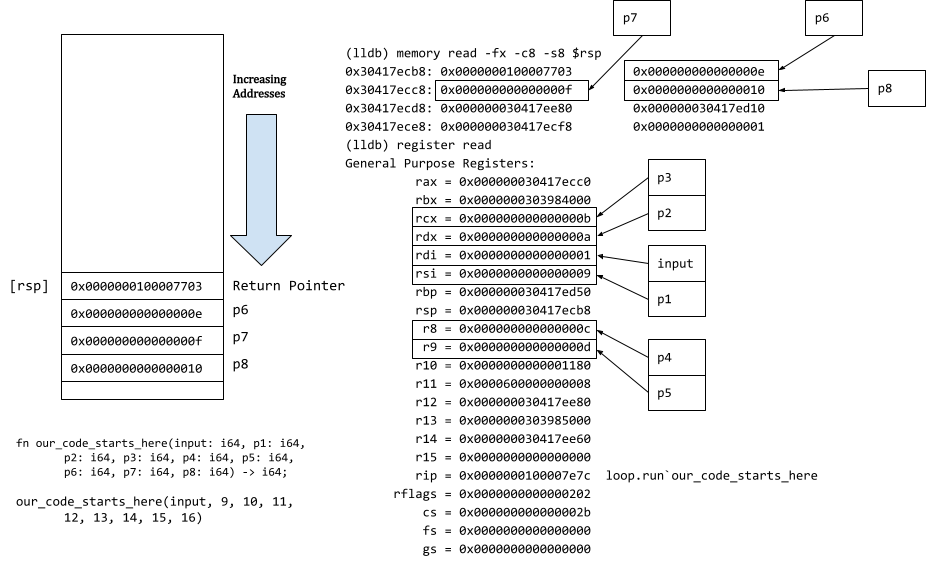
\includegraphics[scale=0.5]{assets/mem_layout.png}
\end{center}
The main takeaways to get are, in x86\_64,
\begin{itemize}
    \item The first 6 arguments are \code{rdi}, \code{rsi}, \code{rdx}, \code{rcx}, \code{r8}, and \code{r9}.
    \item Any remaining arguments will go in order in increasing addresses \textbf{after} \code{[rsp]}, where \code{[rsp]} holds the return pointer.
\end{itemize}

\subsection{Functions \& Their Conventions for Us}
How do we add functions to our programming language? We need to restructure our programming language a bit. First, our program will have the following definition: 
\begin{verbatim}
    <prog> := <defn>* <expr>

    <defn> := (fun (<name> <name>) <expr>)
        | (fun (<name> <name> <name>) <expr>)

    <expr> := ... 
        | (<name> <expr>) 
        | (<name> <expr> <expr>)\end{verbatim}
In particular, 
\begin{itemize}
    \item \code{<prgm>} is what our \code{snek} file will look like. \code{<prgm>} is saying that it takes zero or more function definitions, and then the expression. So, past \code{snek} files had zero function definitions. Now, \code{snek} files can have more than zero function definitions.
    \item In our version of \code{<defn>}, 
    \begin{itemize}
        \item \code{(fun (<name> <name>) <expr>)} means that the function declaration has a \emph{name}, and then one argument after it, and then the following expression. 
        \item \code{(fun (<name> <name> <name>) <expr>)} means that the function declaration has a \emph{name}, and then \emph{two arguments} after the name, and then the following expression.
    \end{itemize}
    \item In \code{<expr>}, not only do we have the usual language features (e.g., numbers, identifiers, binary operations, etc.), but we also have support for calling the above functions. Specifically,
    \begin{itemize}
        \item \code{(<name> <expr>)} calls the function \code{<name>} with a single argument.
        \item \code{(<name> <expr> <expr>)} calls the function \code{<name>} with two arguments.
    \end{itemize}
\end{itemize}
Consider the following code. 
    \begin{verbatim}
    (fun (sumsquare x y)
        (+ (* x x) (* y y)))

    (sumsquare (* 2 input) (+ 30 (* 3 input)))\end{verbatim}
When \code{sumsquare} starts, we should expect the memory and stack to look something like:
\begin{center}
    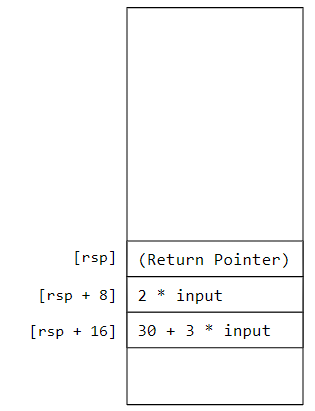
\includegraphics[scale=0.6]{assets/function_mem_layout_dec.png}
\end{center}
In other words, the value of the first argument, $2 \times \code{input}$, when we called the function is in \code{[rsp + 8]}; likewise, the value of the second argument, $3 \times \code{input} + 30$, when we called the function is in \code{[rsp + 16]}. So, in general, how should we generate functions in our assembly code? 
\begin{itemize}
    \item For each function definition, we will generate a label. 
    \item Arguments will be located in the following places: 
    \begin{itemize}
        \item The value of the first argument is located in \code{[rsp + 8]}. 
        \item The value of the second argument is located in \code{[rsp + 16]}.
        \item In general, the value of the $i$th argument is located in \code{[rsp + 8(i + 1)]}.
    \end{itemize}
    This is controlled by the environment used for the body. 
\end{itemize}

Let's try to sketch out the assembly of the above code, where \code{sumsquare} is defined and where it is being called, and the corresponding memory model after running it. 

\begin{center}
    \begin{tabular}{p{3in}|p{3in}}
        \begin{verbatim}
; [rsp + 8] is x 
; [rsp + 16] is y
sumsquare:
    ; TODO 
    ret 

; basically, our main function 
our_code_starts_here:
    ; code for (* 2 input) -> rax 
    mov [rsp - 16], rax 
    ; code for (+ 30 (* 3 input))
    mov [rsp - 24], rax\end{verbatim}
        & \begin{center}
            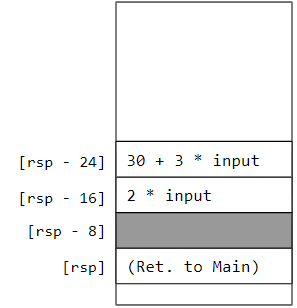
\includegraphics[scale=0.7]{assets/sumsq_arg_order1.png}
        \end{center}
    \end{tabular}
\end{center}

\textbf{Notice} that the order of the arguments isn't correct, so we can't use the arguments as they appear right here. So, we need to do some more moving.

\begin{center}
    \begin{tabular}{p{3in}|p{3in}}
        \begin{verbatim}
; [rsp + 8] is x 
; [rsp + 16] is y
sumsquare:
    ; TODO 
    ret 

; basically, our main function 
our_code_starts_here:
    ; code for (* 2 input) -> rax 
    mov [rsp - 16], rax 
    ; code for (+ 30 (* 3 input))
    mov [rsp - 24], rax
    ; additional moves for args 
    sub rsp, 48 ; 8 * 6
                ; put at "top" of stack
    call sumsquare
    add rsp, 48\end{verbatim}
        & \begin{center}
            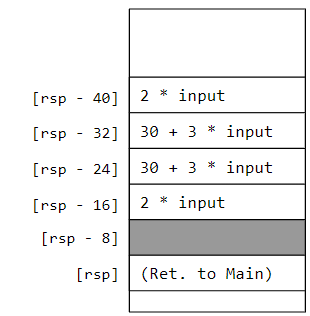
\includegraphics[scale=0.6]{assets/sumsq_arg_order2.png}
        \end{center}
    \end{tabular}
\end{center}
We also may want to \textbf{save} any values that may be caller-saved (e.g., any registers like \code{rdi}). This should be done before doing any additional moves. Basically, we don't want to overwrite anything from a previous stack frame.

\subsection{Improvements and Approaches}
Some small ideas we could think about are: 
\begin{enumerate}
    \item The last argument can avoid copying. This is mainly so we can avoid doing some unnecessary minor work. 
    \item Evaluate arguments in reverse order (last to first). Then, they are in the right place on the stack. 
\end{enumerate}
Both of these run into issues with saving and restoring registers! So, a \textbf{big idea} is to \textbf{pre-allocate stack frames}\footnote{This is what Rust and C does.}. In other words, we move \code{rsp} at the \emph{start} of a function to accommodate \emph{all} local variables. Then, all references are \code{[rsp + \_\_\_]}. The interesting thing to think about is how much we need to move \code{rsp} to accommodate all local variables. Once we figure this out, then we can adjust \code{rsp} as needed. 

\bigskip 

Introducing, the \code{depth} function. This calculates the number of local variables (named or unnamed) are in this expression. This is basically just tracking stack indices. 
\begin{verbatim}
    fn depth(e: &Expr) -> i32 {
        match e {
            Plus(e1, e2) => {
                max(depth(e1), depth(e2) + 1)
            }
            Let(id, val, body) => {
                max(depth(val), depth(body) + 1)
            }
            ...
        }
    }\end{verbatim}
In a \code{Plus} expression, which has \code{e1} and \code{e2}, we're taking the maximum of 
\begin{itemize}
    \item \code{depth(e1)} (Because we don't increase the stack index when we go into \code{e1}), and 
    \item \code{depth(e2) + 1} (Remember that the plus expression makes space for one word, and then reserves that space while it's working on \code{e2}. This corresponds to how we did \code{si + 1} in our compiler.)
\end{itemize}
Analogously, we can say the same for the \code{Let} expression. 

\bigskip 

So, going back to compiling \code{sumsquare}, the first thing we can do is 
\begin{verbatim}
    sumsquare:
        sub rsp, depth(body * 8)
        . 
        . 
        .
        add rsp, depth(body * 8)
        ret\end{verbatim}
Note that all local variables use \code{[rsp + \_\_\_]} in this function. This means less calculations and moving \code{rsp} at each call.
\newpage
\section{Our Calling Convention}
We'll now talk more about the calling conventions we aim to use for our compiler, along with functions in general. Recall, from the previous section, that a \code{snek} program is defined by 
\begin{verbatim}
    <prog> := <defn>* <expr>

    <defn> := (fun (<name> <name>) <expr>)
        | (fun (<name> <name> <name>) <expr>)

    <expr> := ... 
        | (<name> <expr>) 
        | (<name> <expr> <expr>)\end{verbatim}
where \code{<defn>} means that our function declarations can either take one argument, or two arguments, respectively.

\subsection{Caller-Managed Stack Pointer}
An approach for calling functions is to have the caller (i.e., the function that is \emph{calling} a function) manage the stack pointer, \code{rsp}.

\subsubsection{Compiling the Definition}
Let's consider the following Rust code: 
\begin{verbatim}
    fn compile_definition(d: &Definition, labels: &mut i32) -> String {
        match d {
            Fun1(name, arg, body) => {
                ...
            }
            Fun2(name, arg1, arg2, body) => {
                let body_env = hashmap! {
                    arg1.to_string() => -1,
                    arg2.to_string() => -2
                };
                let body_is = compile_expr(body, 2, &body_env, 
                    &String::from(""), labels);
                format!(
                    "{name}:
                    {body_is}
                    ret"
                )
            }
        }
    }\end{verbatim}
This function is designed to compile a function declaration, specifically a function with one and two arguments. Some things to think about: 
\begin{itemize}
    \item Compiling a function is straightforward with this calling convention. All there is to the actual function is 
    \begin{itemize}
        \item The label (perhaps, the name of the function).
        \item The body of the function. 
        \item And then, \code{ret} for returning.
    \end{itemize}
    \item Note that the \emph{environment} is set up so that negative stack indexes are used. This way, the compiler ends up accessing \code{[rsp + X]}, i.e., accessing memory downwards as opposed to upwards. 
    \item In this approach, all the work of manipulating \code{rsp} is done by the \textbf{caller}.
\end{itemize}

\subsubsection{Compiling the Function Calls}
Now, let's look at the code that's responsible for compiling \emph{function calls}.
\begin{verbatim}
    fn compile_expr(
        e: &Expr,
        si: i32,
        env: &HashMap<String, i32>,
        brake: &String,
        l: &mut i32,
    ) -> String {
        match e {
            ...
            Expr::Call2(name, arg1, arg2) => {
                let arg1_is = compile_expr(arg1, si, env, brake, l);
                let arg2_is = compile_expr(arg2, si + 1, env, brake, l);
                let curr_word = si * 8;
                let offset = (si * 8) + (2 * 8);
                // With this setup, the current word will be at [rsp+16], 
                // which is where arg1 is stored. We then want to get rdi
                // at [rsp+16], arg2 at [rsp+8], and arg1 at [rsp], then call
                format!(
                    "
                    {arg1_is}
                    mov [rsp-{curr_word}], rax
                    {arg2_is}
                    sub rsp, {offset}
                    mov rbx, [rsp+16]
                    mov [rsp], rbx
                    mov [rsp+8], rax
                    mov [rsp+16], rdi
                    call {name}
                    mov rdi, [rsp+16]
                    add rsp, {offset}
                "
                )
            }
        }
    }\end{verbatim}
There are some things we need to make sure: 
\begin{itemize}
    \item We need to make sure we set \code{rsp} high enough so that it doesn't interfere with any of the temporary variables. 
    \item We also need to make sure we store the variables (arguments) in the right place before we actually call the function. \code{offset} is defined so that it will be used to move \code{rsp} above where we are, and then subtracting some more words, so we can make room for \code{rdi} and \textbf{two} arguments. 
    \item Note that, even though we have three items (\code{rdi} and the two arguments), we only need to move the stack index up by an additional 16 spaces, hence why we're adding \code{2 * 8}. % TODO why?
\end{itemize}


\subsubsection{Memory Layout}
With the above code for function \emph{calling}, let's look at a memory diagram of what's going on prior to calling a function. We know that \code{curr\_word} is defined as \code{si * 8}.
\begin{center}
    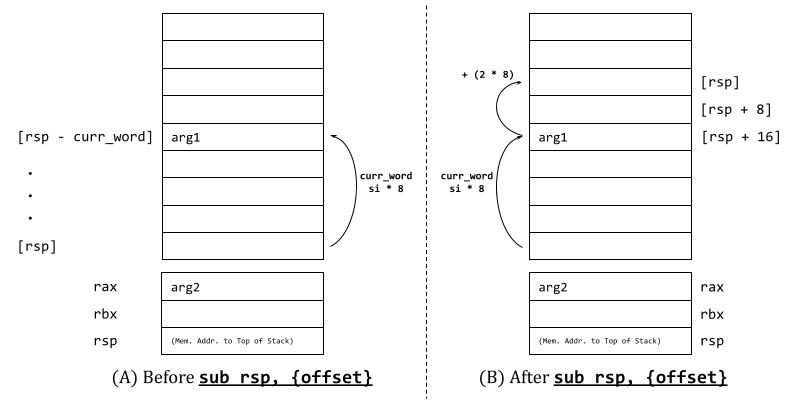
\includegraphics[scale=0.5]{assets/function_stack_mem.png}
\end{center}

So, what's going on? 
\begin{itemize}
    \item Before we call \verb|sub rsp, {offset}|, i.e., in diagram (A), 
    \begin{itemize}
        \item \code{[rsp]} is pointing to some initial return pointer (e.g., at a main expression or some function).
        \item \code{[rsp - curr\_word]} is where we stored \code{arg1} in the stack. Equivalently, \code{arg1} is stored \code{curr\_word} space ``above'' \code{rsp}.
        \item Remember that the result of \code{arg2} is stored in \code{rax}, since that was the last expression that was compiled.
    \end{itemize}

    \item After we call \verb|sub rsp, {offset}|, i.e., in diagram (B), 
    \begin{itemize}
        \item We moved \code{[rsp]} up by \code{(si * 8) + (2 * 8)} spaces, as seen by the two ``jumps'' in the diagram. 
    \end{itemize}
\end{itemize}
Our goal is to put \code{rdi} into \code{[rsp + 16]}, \code{arg2} into \code{[rsp + 8]}, and \code{arg1} into \code{[rsp]}. To make this happen, we need to move a few things around. That's where the following four assembly instructions, 
\begin{verbatim}
    mov rbx, [rsp+16]
    mov [rsp], rbx
    mov [rsp+8], rax
    mov [rsp+16], rdi\end{verbatim}
come from. To see how this works, let's visualize each line. 

\begin{center}
    \begin{tabular}{p{3in}|p{3in}}
        \textbf{After Running} & \textbf{Diagram} \\ 
        \hline 
        (Initial) & 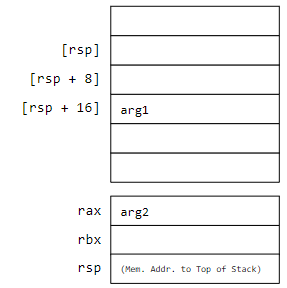
\includegraphics[scale=0.72]{assets/mem1.png} \\ 
        \hline 
        \code{mov rbx, [rsp + 16]} & 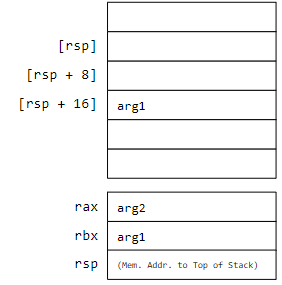
\includegraphics[scale=0.72]{assets/mem2.png} \\ 
        \hline 
        \code{mov [rsp], rbx} & 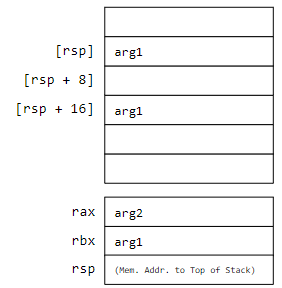
\includegraphics[scale=0.72]{assets/mem3.png} \\ 
        \hline 
        \code{mov [rsp+8], rax} & 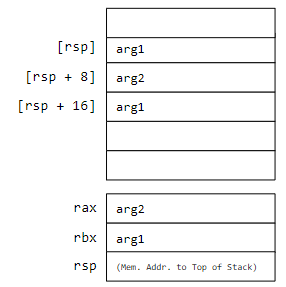
\includegraphics[scale=0.72]{assets/mem4.png} \\ 
        \hline 
        \code{mov, [rsp+16], rdi} &  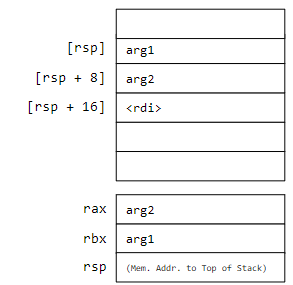
\includegraphics[scale=0.72]{assets/mem5.png} \\ 
    \end{tabular}
\end{center}

\textbf{Remarks:} 
\begin{itemize}
    \item Remember that the above only works for 2 arguments. For arbitrary arguments, the same idea still holds, but you need to generalize it.
    \begin{mdframed}
        \underline{Recall:} \emph{Before} we executed \code{sub rsp, ...}, we can imagine that \code{arg1} is at \code{[rsp - si * 8]}, \code{arg2} is at \code{[rsp - si * 8 - 8]}, \code{arg3} is at \code{[rsp - si * 8 - 16]}, and so on until \code{argN-1} is at \code{[rsp - si * 8 - 8(N - 1)]}. As usual, \code{rax} will hold \code{argN}.
    \end{mdframed}
    After we move \code{[rsp]}, we can expect \code{argN-1} to be at \code{[rsp + 16]}, \code{argN-2} to be at \code{[rsp + 24]}, and so on, with \code{arg1} being at \code{[rsp + 8(N + 1)]}. As usual, \code{rax} holds \code{argN}.
    
    \item \code{rdi} is a caller-saved register, hence why we're purposely saving it. 
    \item In this calling convention, as one might have guessed, we're putting everything on the stack. 
    \item While function arguments need positive offsets from \code{rsp}, \textbf{local variables} (temporaries) still use negative offsets from \code{rsp}. 
\end{itemize}
Now, after we do the \code{call} instruction, the memory diagram looks like 
\begin{center}
    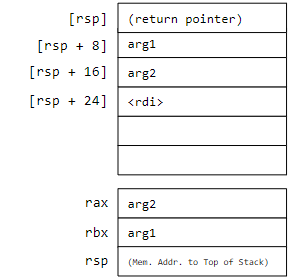
\includegraphics[scale=0.9]{assets/mem6.png}
\end{center}
In other words, the \code{call} instruction will move \code{rsp} up and write the return pointer into that word. At that point, it's clear that \code{arg1} and \code{arg2} are in the correct offsets.

\subsection{Callee-Managed Stack Pointer}
Suppose, instead, we want to have the function itself manage the stack pointer by moving it sufficiently enough. Then, at the start of a function call, suppose the memory diagram looks like this: 
\begin{center}
    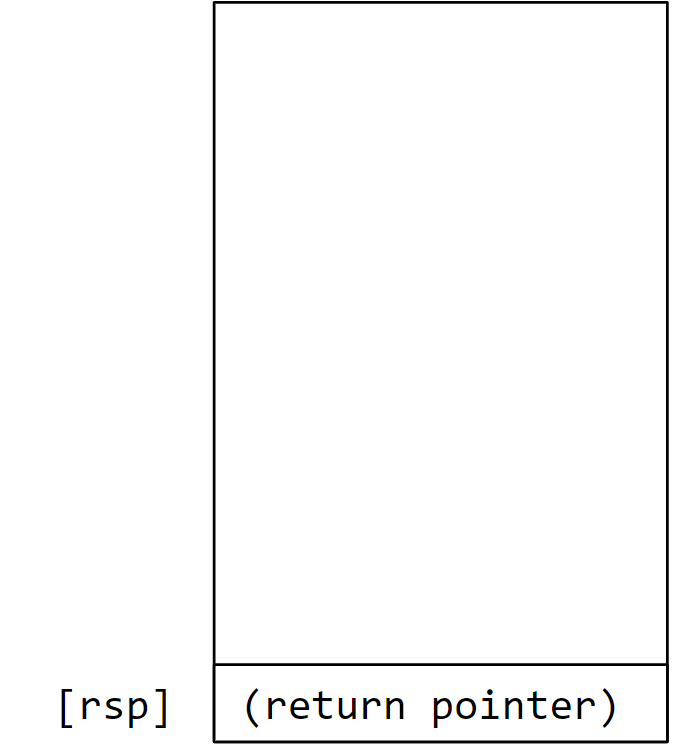
\includegraphics[scale=0.3]{assets/callee_stack_mnged_init.png}
\end{center}
Under this assumption where the callee manages the stack pointer, the first thing the function will do is \code{sub rsp} so that there's enough space for all local variables. That is, we should move \code{[rsp]} so that we end up with a memory diagram that looks like 
\begin{center}
    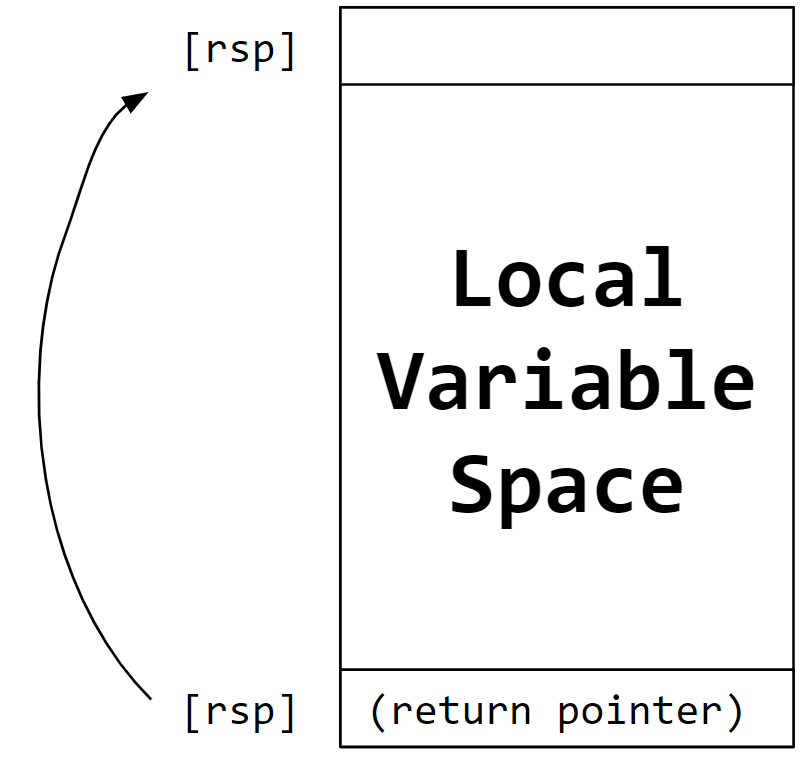
\includegraphics[scale=0.3]{assets/callee_stack_mnged.png}
\end{center}
Then, all lookups, including for argument and local variables, will have its location in the stack be positive offsets from \code{rsp}. There are some advantages to doing this, especially in relation to garbage collection.

\subsubsection{The Depth Function}
First, we need to know how many local variables are needed in the body of a function so we know how much we need to move \code{rsp} by. We can use the \code{depth} function to calculate the maximum stack index needed in an expression to store all local variables and temporaries. 

\bigskip 

Using the power of ChatGPT, along with some corrections, we have the following implementation:
\begin{verbatim}
fn depth(e: &Expr) -> i32 {
    match e {
        Expr::Num(_) => 0,
        Expr::True => 0,
        Expr::False => 0,
        Expr::Add1(expr) => depth(expr),
        Expr::Plus(expr1, expr2) => depth(expr1).max(depth(expr2) + 1),
        Expr::Let(_, expr1, expr2) => depth(expr1).max(depth(expr2) + 1),
        Expr::Id(_) => 0,
        Expr::Eq(expr1, expr2) => depth(expr1).max(depth(expr2) + 1),
        Expr::If(expr1, expr2, expr3) => {
            depth(expr1).max(depth(expr2)).max(depth(expr3))
        },
        Expr::Loop(expr) => depth(expr),
        Expr::Block(exprs) => exprs.iter().map(|expr| depth(expr)).max().unwrap_or(0),
        Expr::Break(expr) => depth(expr),
        Expr::Print(expr) => depth(expr),
        Expr::Set(_, expr) => depth(expr),
        Expr::Call1(_, expr) => depth(expr),
        Expr::Call2(_, expr1, expr2) => depth(expr1).max(depth(expr2) + 1),
    }
}\end{verbatim}

\subsubsection{Compiling the Definition}
With this in mind, we have 
\begin{verbatim}
    fn compile_definition(d: &Definition, labels: &mut i32) -> String {
        match d {
            Fun1(name, arg, body) => {
                ...
            }
            Fun2(name, arg1, arg2, body) => {
                let depth = depth(body);
                let offset = depth * 8;
                let body_env = hashmap! {
                    arg1.to_string() => depth + 1,
                    arg2.to_string() => depth + 2
                };
                let body_is = compile_expr(body, 0, &body_env, 
                    &String::from(""), labels);
                format!(
                    "{name}:
                    sub rsp, {offset}
                    {body_is}
                    add rsp, {offset}
                    ret"
                )
            }
        }
    }\end{verbatim}
We also need to do the same thing with the main expression (the main program):
\begin{verbatim}
    sub rsp, {offset}
    {main}
    add rsp, {offset}\end{verbatim}
where \code{offset} is defined by: 
\begin{verbatim}
    let depth = depth(&p.main); // p.main -> main program
    let offset = depth * 8;\end{verbatim}

\subsubsection{Changing Offsets in Code}
Recall how, before this section, any offsets we used were negative offsets (e.g., \verb|mov [rsp - {offset}], rax|). With this change, we now can use \textbf{positive offsets} (e.g., \verb|mov [rsp + {offset}], rax|). This scheme is similar to what most compilers like Rust, \code{g++}, and so on use. 
\newpage
\section{Introduction to Recursion}
In this section, we'll talk about recursion. Note that, in our examples, we'll assume that the callee manages (i.e., moves) the stack pointer. In particular, this means everything will have a positive offset from \code{rsp}.

\subsection{Recursive Sum Example}
Let's consider the following code:
\begin{verbatim}
(fun (sumrec num)
    (if (= num 0)
        0
        (+ num (sumrec (+ num -1)))
    )
)\end{verbatim}
This program simply performs $1 + 2 + 3 + \hdots + \code{num}$. The generated assembly would look something like what is shown below. 
\begin{verbatim}
sumrec:
    sub rsp, 16
    mov rax, [rsp + 24]
    ... if (= num 0)
    cmp rax, 1
    je ifelse_1
         mov rax, 0
         jmp ifend_0
    ifelse_1:
         ... put temp num on stack for LHS
         mov [rsp + 0], rax
         mov rax, [rsp + 24]
         ... (+ num -1) stored in rax
         ... now do 1-arg calling conv
         sub rsp, 16
         mov [rsp], rax
         mov [rsp+8], rdi
         call sumrec
         mov rdi, [rsp+8]
         add rsp, 16
         ... do addition on the waiting num ...
         add rax, [rsp + 0]
    ifend_0:
    
    add rsp, 16
    ret\end{verbatim}
Note that only relevant assembly is shown. Some things to point out: 
\begin{itemize}
    \item In the second assembly line, \code{sub rsp, 16}, the \code{16} is the \emph{depth} that we calculated. 
    \item In the lines before the recursive call, i.e., 
    \begin{verbatim}
        sub rsp, 16
        mov [rsp], rax
        mov [rsp+8], rdi
        call sumrec\end{verbatim}
    we're moving the arguments into the correct position in memory so the recursive call can make use of them. 
    \item When we run a \code{call} instruction, \code{rsp} is moved up one word and the return pointer to the next line of instruction (program counter) is put in that location in memory (where \code{rsp} is pointing to). 
\end{itemize}
To see how the memory looks when each line of assembly is executed, see \code{Lec12Trace.pdf}.




\subsection{Second Recursive Sum Example}
Let's rewrite the recursive sum example a bit.  
\begin{verbatim}
(fun (sumrec num sofar)
    (if (= num 0)
        sofar 
        (sumrec (+ num -1) (+ sofar num))
    )
)\end{verbatim}
The generated assembly might look like 
\begin{verbatim}
sumrec:
    sub rsp, 16
    
    mov rax, [rsp + 24]
    mov [rsp + 0], rax
    ... if (= num 0)  
    cmp rax, 1
    je ifelse_1
        mov rax, [rsp + 32]
        jmp ifend_0
    ifelse_1:
        mov rax, [rsp + 24]
        ... add -1 to num, store on stack as tmp ...
        mov [rsp + 0], rax

        mov rax, [rsp + 32]
        ... add sofar to num, store in rax ...
        add rax, [rsp + 8]
  
        ... 2-arg calling convention from class ...
        sub rsp, 24
        mov rbx, [rsp+24]
        mov [rsp], rbx
        mov [rsp+8], rax
        mov [rsp+16], rdi
        call sumrec             ; (A)
        mov rdi, [rsp+16]       ; (B)
        add rsp, 24             ; (C)
    
    ifend_0:
    add rsp, 16                 ; (C)
    ret                         ; (D)\end{verbatim}
An interesting thing to note is that, after reaching the base case, there's no additional calculation that needs to be made. In particular, the steps after returning is 
\begin{enumerate}[(a)]
    \item Move \code{rsp} back. Remember that, after \code{call} is done (i.e., when \code{ret} is executed), \code{rsp} is moved back one word.
    \item Restore \code{rdi}.
    \item Move \code{rsp} back more. 
    \item Return!
\end{enumerate}
No local variables or arguments were accessed.
\newpage
\section{Introduction to Tail Recursion}
Let's consider the following function:
\begin{verbatim}
    (fun (sumrec num sofar)
        (if (= num 0)
            sofar 
            (sumrec (+ num -1) (+ sofar num))
        )
    )\end{verbatim}
This function is in tail position: that is, after the recursive call, we don't need to do any additional computations. The assembly representation, is shown to the left. On the right, the stack frame when \code{(subrec 3 0)} is evaluated is shown, at the point when the base case is about to be executed. 
\begin{center}
    \begin{tabular}{p{3in} p{3in}}
        \begin{verbatim}
    sumrec:
        sub rsp, 16
        
        mov rax, [rsp + 24]
        mov [rsp + 0], rax
        ... if (= num 0)  
        cmp rax, 1
        je ifelse_1
            mov rax, [rsp + 32]
            jmp ifend_0
        ifelse_1:
            mov rax, [rsp + 24]
            ... add -1 to num, 
            ... store on stack as tmp
            mov [rsp + 0], rax
    
            mov rax, [rsp + 32]
            ... add sofar to num, 
            ... store in rax
            add rax, [rsp + 8]
      
            ... 2-arg calling 
            ... convention from class
            sub rsp, 24
            mov rbx, [rsp+24]
            mov [rsp], rbx
            mov [rsp+8], rax
            mov [rsp+16], rdi
            call sumrec 
        --> mov rdi, [rsp+16]
            add rsp, 24 
        
        ifend_0:
        add rsp, 16
        ret\end{verbatim}
        & \begin{center}
            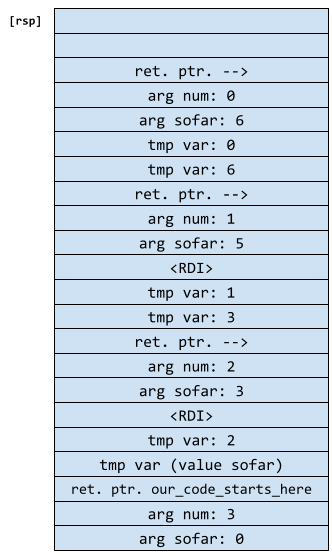
\includegraphics[scale=0.6]{assets/tail_rec_diagram.png}
        \end{center}
    \end{tabular}
\end{center}


\begin{mdframed}
    (Exercise.) What will \code{RAX} be after each return pointer? 

    \begin{mdframed}
        \code{RAX} will be \textbf{6}. There are two ways you can tell: 
        \begin{itemize}
            \item In the code itself, the base case just returns the \code{sofar} argument. Intuitively, this means that this function should return 6 for all subcalls, implying \code{rax} has 6 at every return pointer. 
            \item Additionally, when looking at the generated assembly, notice the \code{move rax, [rsp + 32]} instruction. \code{[rsp + 32]} points to the value \code{sofar}, 6. Pair this with when we look at the instructions after the \code{call} instruction (which is where the program returns to after \code{ret} is executed), notice that there's no additional move instructions to \code{rax}. 
        \end{itemize}
    \end{mdframed}
\end{mdframed}
\textbf{Remark:} There are several things to notice:
\begin{itemize}
    \item there's no use of local variables or arguments following the \code{call} instruction. 
    \item there are no changes to \code{rax} after the \code{call} instruction.
\end{itemize}
These observations means that we can reuse the space that we set up for the function call to perform all operations. In other words, we can use one stack frame's worth of space for the \emph{entire} computation! Basically, we're using more space than we need. 

\subsection{Restructuring the Assembly}
Instead of the \code{call} instruction above, what should we do to replace the instructions so that the new instructions overwrite the current arguments with the new arguments and ``re-use'' the stack frame? 

\bigskip 

We can preemptively add to \code{rsp} to ``undo'' the \code{sub} at the beginning of the function. That is, 
\begin{center}
    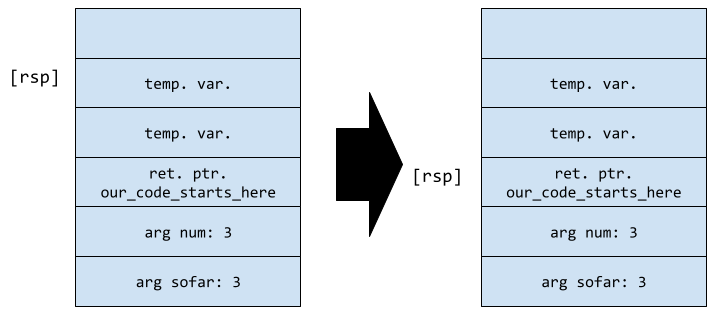
\includegraphics[scale=0.5]{assets/tail_call_2.png}
\end{center}
So, we can write the following assembly:
\begin{verbatim}
    add rsp, 16 
    mov rbx, [rsp - 16]
    mov [rsp + 8], rbx 
    mov [rsp + 16], rax 
    jmp sumrec\end{verbatim}
Notice how we have an \emph{unconditional jump} to \code{sumrec}, as opposed to a \code{call} instruction. This is important, because this effectively means we have a \textbf{loop}!
\begin{center}
    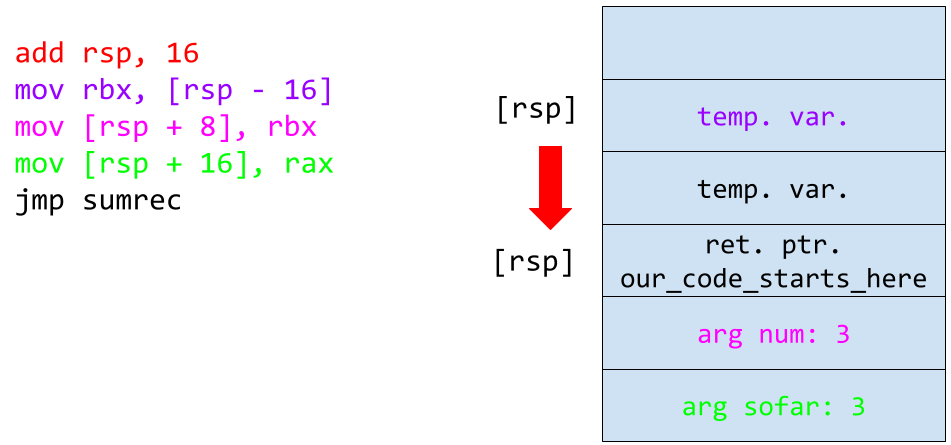
\includegraphics[scale=0.4]{assets/tail_call_3.png}
\end{center}
This process is known as \textbf{proper tail calls}. We effectively re-use the stack from when the ``last thing'' is a function call (what would have been a separate function call with its own stack frame is now a separate ``function call'' re-using the same stack frame from the current ``function call.'').

\subsection{Tail Call Positions}
When is an expression in tail call position? How does the compiler know when it is in tail call position? A few things: 
\begin{itemize}
    \item Anything where we generate instructions that work with the result of a subexpression is not in tail call.  
    \item Essentially, if you work with \code{rax} or store the value after a recursive call to the compile function, that recursive function call cannot be in tail call position. If you don't do anything with it and rely on the answer being in \code{rax} after making the recursive call, then it's in tail position.
\end{itemize}
So, with this in mind: 
\begin{itemize}
    \item \code{Add1}: not in tail call position (adds 1 to \code{rax}). 
    \item \code{Eq}: not in tail call position (needs to store \code{rax} somewhere before compiling the second expression so we can compare them).
    \item \code{Plus}: not in tail call position (needs to store \code{rax} somewhere so we can add to \code{rax} later).
    \item \code{Let}: the value associated with the binding cannot be in tail position, but the body of the \code{let}-expression \emph{can} be in tail position (provided that any preceding calls are in tail position as well).
    \item \code{If}: the conditional expression cannot be in tail position, but the then/else expressions can be in tail position (provided that any preceding calls are in tail position as well).
    \item \code{Block}: only the last expression in a block can be in tail position; the other expressions cannot be in tail position. 
    \item \code{Break}/\code{Loop}: they \emph{generally} cannot be in tail call position (there are special cases, though).
\end{itemize}
In a function call, the arguments cannot be in tail-call position. Note that the body of the expression is where we compile tail call position code or regular code based on whether we're in tail call position. 

\bigskip 

In other words, at the beginning of compilation, we assume that we're in tail call position. As we compile each expression, we might ``lose'' that tail call position. We can never get it back once lost in that subexpression.
\newpage
\section{Structured Data: Pairs}
In this section, we'll introduce \textbf{structured data} to our programming language. In particular, we'll introduce \textbf{pairs}, which is essentially a two-element tuple where both elements can be anything -- numbers or pairs.

\subsection{Pair Expressions}
Our language now has the following syntax: 
\begin{verbatim}
    expr := ... | (pair <expr> <expr>) | (fst <expr>) | (snd <expr>) | nil\end{verbatim}
Here, \code{pair} defines a pair of expressions. \code{fst} and \code{snd} returns the first and second element of a pair\footnote{Although \code{fst} and \code{snd} takes any expressions, it expects a pair expression.}, respectively.

\begin{mdframed}
    (Exercise.) What will the following program evaluate to? 
    \begin{verbatim}
        (fun (inc lst)
            (if (= lst nil)
                nil
                (pair (+ (fst lst) 1) (inc (snd lst)))
            )
        )
    
    (inc (pair 70 (pair 800 nil)))\end{verbatim}

    \begin{mdframed}
        The answer is \code{(71, (801, nil))}. In this function, we first check if the given pair is \code{nil}; if it is, return \code{nil}. Otherwise, we create a new pair where the first expression is just the first element of the original pair incremented by 1, and the second element is the result of recursively calling \code{inc} on the second element of the original pair.

        \bigskip 

        We can think of the \code{(snd lst)} as the \emph{rest of the list}. 
    \end{mdframed}
\end{mdframed}

\begin{mdframed}
    (Exercise.) What will the following program evaluate to? 
    \begin{verbatim}
        (fun (sum lst)
            (let (total 0)
                (loop 
                    (if (= lst nil) 
                        (break total) 
                        (block
                            (set! total (+ total (fst lst)))
                            (set! lst (snd lst)) 
                        )
                    )
                )
            )
        )
    
        (sum (pair 70 (pair 800 nil)))\end{verbatim}
    
    \begin{mdframed}
        The answer is 870. This program iterates through each element of the pair, getting its value and adding it to \code{total}. In particular, if we ran the program, we see that 
        \begin{verbatim}        
    Expression                          (fst lst)       Total
    (pair 70 (pair 800 nil))            70              70
    (pair 800 nil)                      800             870 
    nil                                 -               -\end{verbatim}
    \end{mdframed}
\end{mdframed}

\subsection{Representing Pairs}
Recall that we used a tagging system, where we dedicated one bit, to differentiate numbers and booleans. However, with a new type, we need to rethink the tagging system. 

\bigskip 

Our tagging system will now consist of the following:
\begin{itemize}
    \item \textbf{Numbers} will still use \code{0} as its tag value.
    \item \textbf{Booleans} will use \code{11} as its tag value. 
    \begin{itemize}
        \item \code{true} will be represented in binary as \code{111} (7).
        \item \code{false} will be represented in binary as \code{011} (3).
    \end{itemize}
    \item \textbf{Pairs} will use \code{01} as its tag value. 
    \item \textbf{Nil} will use \code{1} as its tag value.
\end{itemize}
With a tagging system in hand, how do we represent pairs themselves? One approach is as follows: 
\begin{itemize}
    \item An idea is to store each of the pair's value as 31-bits. For example, to represent 2 numbers, we would represent the first number as 31 bits, and the next number as another 31 bits, with the tag value being 2 bits. 
    \item \textbf{However}, this won't really work if we have nested pairs. For example, if we have a pair with pairs as its element, then how do we represent this? 
\end{itemize}
Another thing we can think about is heap allocation. 

\subsection{Compiler Design}
As implied, we'll have to allocate pair element on the \textbf{heap} (we'll need to work with the Rust runtime for this). So, our representation is that the pair's value will be a 62-bit address on the heap. 

\bigskip 

How do we know \emph{where} to allocate pair elements on the heap? An idea is to dedicate a register that just keeps track of the current heap location. In our class, we'll use \code{r15} for our purposes. With this in mind, here are a few assumptions we will be making:
\begin{itemize}
    \item \code{r15} is expected to keep growing for now; it's not like \code{rsp} where it can increase or decrease depending on how stack space is used. 
    \item \code{r15} only refers to available memory, never used memory. 
    \item \code{r15} will be 16-byte aligned (it will end with \code{0000})
\end{itemize}
With this in mind, how do we modify our compiler to support pairs? A sketch of an implementation we'll use is as follows: 
\begin{verbatim}
    Pair(e1, e2) => {
        let fst = compile_expr(e1, ...);
        let snd = compile_expr(e2 ...);
        // e1 will be somewhere in [rsp], e2 in rax 
        format!("
            {fst}
            {snd}
            mov [r15 + 8], rax 
            mov rbx, [rsp + offset]
            mov [r15], r15
            mov rax, r15 
            add rax, 1 
            add r15, 16
        ")
    }\end{verbatim}
\textbf{Remarks:} 
\begin{itemize}
    \item We should probably first check and see if we have space left before allocating. We didn't do this part yet.  
    \item Note that we move \code{rax} into \code{[r15 + 8]} (and not \code{[r15]}) because \code{rax} has the value of the \emph{second} element of the pair, not the first. 
    \item \code{mov rax, r15} and \code{add rax, 1} is designed to put the location in heap of the pair's values into \code{rax} and then add 1 to \code{rax} for tagging purposes. Note that we can add \code{1} to \code{rax} like this because we know that \code{r15} will end with \code{0000} (this is one of the assumptions we made). 
    \item \code{add r15, 16} moves \code{r15} by 2 words, thus ensuring that it's always pointing to free memory in the heap. 
\end{itemize}
As one might have suspected, once we execute a pair, it should return the memory location to that pair. 

\subsection{Heap Allocation}
We actually have two things we need to do here: 
\begin{itemize}
    \item We need to create some sort of a \emph{heap} that our compiler can use to store pair values. Once we create 
    \item We need to put the heap pointer into \code{r15}.
\end{itemize}
Let's think about some ideas for how we can set the heap up.
\begin{itemize}
    \item One idea is to set \code{r15} to \verb|rsp - {a lot}|. In other words, if we move \code{rsp} very high up, then we can use \code{r15} as the ``heap'' pointer. \textbf{However}, let's think about the process layout:
    \begin{center}
        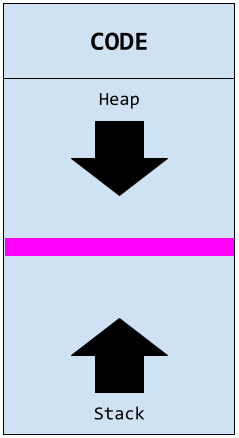
\includegraphics[scale=0.4]{assets/process_layout.png}
    \end{center}
    The typical convention is that the heap grows downwards and the stack grows upwards. In around the middle of memory (denoted by the pink rectangle), there's some special addresses where touching them will result in an error (heap overflows and stack overflows). So, if we set \code{rsp} high enough, then we might either hit that special address, or if we have a depth-heavy recursion\footnote{Since this can hit our proposed ``heap'' space.}, or if we somehow point \code{r15} to the heap space\footnote{Since this is where Rust might allocate memory, so we might end up overwriting memory that Rust needs.}, then we'll be in trouble. 

    \item We can also call Rust's equivalent of \code{malloc}, and use its value\footnote{\code{malloc} gives us the address to some allocated memory in the heap.}. In particular, 
    \begin{itemize}
        \item Call \code{malloc} for each pair\footnote{Note that heap size is \emph{unknowable} iin general \textbf{statically}.}, or 
        \item One \emph{big} \code{malloc}.
    \end{itemize}
    The suggestion we'll use is similar to having a \textbf{big} \code{malloc}. This has the added benefit of being easy to \code{free} at the end. 
\end{itemize}

\subsection{Modifying Our Rust Code}
Now, we need to modify our Rust code to account for these changes. 

\subsubsection{Modifying the Runtime}
In \code{runtime.rs}, we'll essentially do the following:
\begin{verbatim}
    fn main() {
        let args = ...;
        let input = parse_arg(&args);
        let mut memory = Vec::with_capacity(100_000);       // New!
        let buffer: *mut u64 = memory.as_mut_ptr();         // New! 
        let i: i64 = unsafe {
            our_code_starts_here(input, buffer); 
        };

        snek_print(i);
    }\end{verbatim}
Essentially, we'll create a vector with an initial capacity of \code{100\_000} elements. This will represent our heap. Then, we can get a pointer to that vector, and then pass that pointer into our generated assembly. This means our signature for \code{our\_code\_starts\_here} will look like:
\begin{verbatim}
    extern "C" {
        #[link_name = "\x01our_code_starts_here"]
        fn our_code_starts_here(input: i64, buffer: *mut u64) -> i64;
    }\end{verbatim}

\subsubsection{The Generated Assembly}
In our generated assembly, we'll have 
\begin{verbatim}
    our_code_starts_here:
        mov r15, rsi
        ...\end{verbatim}
Here, \code{rsi} represents the \emph{second} argument\footnote{Recall the x86\_64 calling convention.}. 

\subsubsection{Printing Values}
Finally, we need to adjust the \code{snek\_print} function. In particular, our function now needs to account for the fact that it can either receive 
\begin{itemize}
    \item a number (with tag \code{0}).
    \item a boolean (with tag \code{11}).
    \item a pair (with tag \code{01}).
    \item \code{nil} (with tag \code{1}).
\end{itemize}
With this in mind, we have 
\begin{verbatim}
    fn snek_str(val: i64) -> String {
        if val == 7 { "true".to_owned()} 
        else if val == 3 { "false".to_owned() } 
        else if val % 2 == 0 { format!("{}", val >> 1) } 
        else if val == 1 { "nil".to_owned() } 
        else if val & 1 == 1 {
            let addr = (val - 1) as *const i64; 
            let fst = unsafe { *addr };
            let snd = unsafe { *addr.offset(1) };
            format!("(pair {} {})", snek_str(fst), snek_str(snd))
        } else { format!("unknown value: {val}") }
    }

    #[export_name = "\x01snek_print"]
    fn snek_print(val: i64) -> i64 {
        println!("{}", snek_str(val));
        val 
    }\end{verbatim}
Note that \code{offset} is used so we don't need to do direct pointer arithmetic\footnote{We're looking at the memory location directly next to the current memory location since pairs are contiguous.}. Note that we'll need to do some work printing parentheses and whatnot.

\subsection{Memory Representation}
Suppose we have the following program: 
\begin{verbatim}
    (pair 5 (pair 6 (pair 7 nil)))\end{verbatim}
The way we compile this is to first compile the left-most part of the pair (\code{5}), and then the right-most part of the pair (the rest of the pair, in this case). In particular,
\begin{itemize}
    \item The instructions for any nested expressions get evaluated before we move those values onto the heap for the current pair.
    \begin{mdframed}
        In this program's case, we evaluate \code{5} first, and then \code{6}, and then \code{7}. We put all of them on the stack first. \emph{Then}, we put 7 onto the heap first (while \code{6} and \code{5} wait). 
    \end{mdframed}
    
    \item The first pair that gets allocated is the innermost pair. 
\end{itemize}
If we assume left-to-right evaluation order, then \code{7} goes on the heap first. In this sense, allocation happens inside-out. In any case, in the heap, we expect the memory layout to look like
\begin{center}
    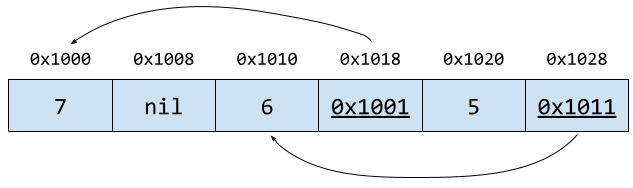
\includegraphics[scale=0.67]{assets/pair_heap.png}
\end{center}
\textbf{Remarks:} 
\begin{itemize}
    \item We have \code{0x1001} and \code{0x1011} (instead of \code{0x1000} and \code{0x1010}) because we use \code{0x01} as the tag value for the pair.
    \item Note that, in our implementation of the compiler, we're actually going to store the integer multiplied by 2 (e.g., 14, 12, and 10, respectively), since in memory we're storing the \emph{tagged} value. In this example, we're just showing the integers as is (with no tagging).
    \item This program would evaluate to \code{0x1021}, since this is the memory address to the first element in the pair. 
\end{itemize}

\begin{mdframed}
    Another way to think about this is as follows: if we wanted to translate this program into something like Python, syntactically this would look like 
    \begin{verbatim}
        p1 = (7, nil);
        p2 = (6, p1);
        p3 = (5. p2);\end{verbatim}
    We had to \emph{allocate} memory for \code{p1} (the innermost pair), and then allocate memory for \code{p2}, and then finally for \code{p3}.
\end{mdframed}

Let's now suppose we have the following program:
\begin{verbatim}
    (fun (inc lst)
        (if (= lst nil)
            nil
            (pair (+ (fst lst) 1) (inc (snd lst)))
        )
    )

    (inc (pair 70 (pair 800 nil)))\end{verbatim}
The heap diagram might look something like 
\begin{center}
    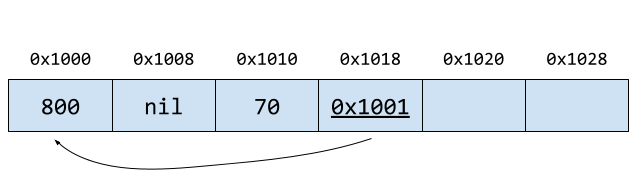
\includegraphics[scale=0.6]{assets/pair_heap2.png}
\end{center}
Here, the result of \code{(pair 70 (pair 800 nil))} is \code{0x1011}, so \code{0x1011} is passed into the \code{inc} function. If we look at the function itself, we can see that the function itself will return the same pair, pair, nil structure.
\begin{center}
    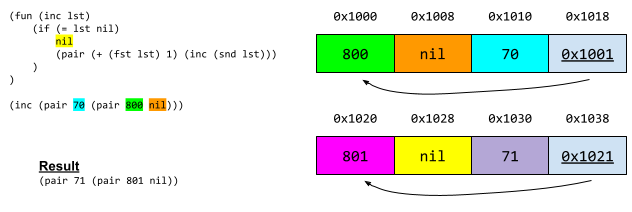
\includegraphics[scale=0.73]{assets/pair_heap3.png}
\end{center}
And, in this exmaple. this function would return \code{0x1031}, the address to the newly created pair.

\subsection{Equality}
Let's consider the following program: 
\begin{verbatim}
    (let (point1 (pair 6 5))
        (let (point2 (pair 6 5))
            (block 
                (print (= point1 point1))                       // A
                (print (= point1 point2))                       // B
                (let (pointpair1 (pair point1 point2))
                    (let (pointpair2 (pair point1 point2))
                        (block 
                            (print (= pointpair2 pointpair2))   // C
                            (print (= pointpair1 pointpair2))   // D
                        )
                    )
                )
            )
        )
    )\end{verbatim}
We now need to decide what this program should print. More specifically, however, we need to figure out how equality of pairs will work. This introduces two types of equalities:
\begin{itemize}
    \item \textbf{Reference equality:} are the two operands referring to the same memory address? For example, in Python, this is \code{==}.
    \item \textbf{Structural equality:} are the two operands equal when considering their structures? For example, in Python, this is \code{is}.
\end{itemize}
With this in mind, we have 
\begin{center}
    \begin{tabular}{|c|c|c|}
        \hline 
        Statement & Reference Equality & Structural Equality \\ 
        \hline
        A & \code{true} & \code{true} \\ 
        B & \code{false} & \code{true} \\ 
        C & \code{true} & \code{true} \\ 
        D & \code{false} & \code{true} \\ 
        \hline  
    \end{tabular}
\end{center}
Note statements (C) and (D); if we want structural equality, we probably want to do \emph{recursive structural equality!} 

\subsection{Revisiting Print}
Let's suppose we have the following program:
\begin{verbatim}
    (let (p (pair 1 2))
        (block 
            (setfst! p p)
            (print p)
        )
    )\end{verbatim}
One thing we should note is that we have a \textbf{cycle} in the sense that the pair is referring to itself. Therefore, if we tried to \code{print} the pair, we would end up with infinite recursion since we would constantly recurse through the first element of the pair. 

\bigskip 

To fix this, we should consider checking if we've \emph{seen} the pair before. If we've seen it, we can print something indicating that a cycle is detected. Otherwise, we can print out the pair as normal. 
\begin{verbatim}
    fn snek_str(val: i64, seen: &mut Vec<i64>) -> String {
        if val == 7 { "true".to_owned()} 
        else if val == 3 { "false".to_owned() } 
        else if val % 2 == 0 { format!("{}", val >> 1) } 
        else if val == 1 { "nil".to_owned() } 
        else if val & 1 == 1 {
            if seen.contains(&val) { return "...".to_owned() }
            seen.push(val);
            let addr = (val - 1) as *const i64; 
            let fst = unsafe { *addr };
            let snd = unsafe { *addr.offset(1) };
            let v = format!("(pair {} {})", snek_str(fst), snek_str(snd));
            seen.pop();
            v 
        } else { format!("unknown value: {val}") }
    }

    #[export_name = "\x01snek_print"]
    fn snek_print(val: i64) -> i64 {
        println!("{}", snek_str(val, &mut vec![]));
        val 
    }\end{verbatim}

\subsection{A Brief Sketch of Equality}
Given two pairs, how can we check if they are equal? We can use the following Rust implementation, 
\begin{verbatim}
    fn snek_eq_helper(val1: i64, val2: i64, seen: &mut Vec<(i64, i64)>) -> bool {
        if seen.contains(&(val1, val2)) { return true }

        seen.push((val1, val2));
        // continue on.
    }\end{verbatim}
The idea is that if we come across the same two cycles, we can assume that they're equal and return. Otherwise, we can evaluate the pairs as usual.
\newpage
\section{Garbage Collection}
Now that we're working with memory in the heap, let's suppose we \emph{don't} have a lot of memory to work with. In this case, we need to think about \emph{garbage collection} as a way to get rid of unused memory so we can allocate memory for useful things. 

\subsection{Motivation}
Let's take a look at two examples to get an idea of what we're working with. 

\subsubsection{Motivation 1: Basic Garbage}
Recall the following code from class: 
\begin{verbatim}
(let (x (pair 1 2))
    (let (y (let (tmp (pair 10 20)) (+ (fst tmp) (snd tmp))))
        (let (p0 (+ (fst x) y))
            (let (p1 (+ (snd x) y))
                (pair p0 p1)
            )
        )
    )
)\end{verbatim}

After creating the final pair, the memory diagram looks like\footnote{For the sake of conciseness, we're showing the numbers without their tagged representation.}\footnote{Also, the \code{tmp} to \code{y} arrow indicates that we're \emph{reusing} that space.} 
\begin{center}
    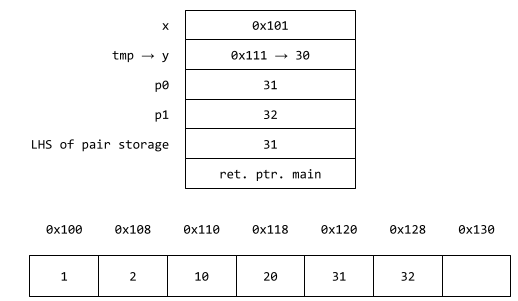
\includegraphics[scale=0.6]{assets/stackHeapPairGC1.png}
\end{center}
Here, the stack is the top diagram while the heap is the bottom diagram. Note that \code{rax}\footnote{Which is storing the answer to our program} is \code{0x121}, and \code{r15}\footnote{Recall that \code{r15} will always point to the next available word in the heap} is \code{0x130}. 

\bigskip 

\textbf{Now, let's suppose} our heap only has five available words. \code{rax} will hold the result of \code{(+ (snd x) y)} (i.e., result of addition, which is a number). Immediately, we should notice that 
\begin{itemize}
    \item We don't have enough memory to allocate for the final pair!
    \item More importantly, however, the values in the heap at location \code{0x110} and \code{0x118} are \textbf{garbage}. Nothing in the stack (or a register) is referring to these values!  
\end{itemize}
To clarify, the idea is that any memory that is not reachable from the stack (or any registers) is considered garbage and can be reused. So, our goal is to get rid of the garbage so we have enough memory to allocate for the final pair. With this said, a high-level implementation of a basic garbage collector would look something like this. 
\begin{center}
    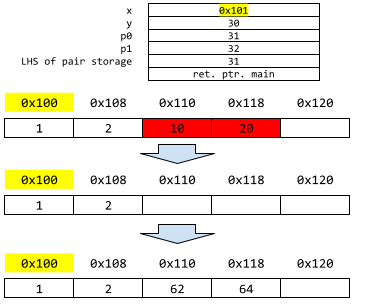
\includegraphics[scale=0.7]{assets/stackHeapPairGCFix1.png}
\end{center}
So here's what's going on:
\begin{itemize}
    \item We've determined that the stuff at \code{0x110} and \code{0x118} are garbage, so we can get rid of them. 
    \item After that, we can \emph{compact the heap}, essentially moving \code{r15} back to \code{0x110}. After that, we can allocate memory for our next pair. 
    \item This gives us the desired result, with \code{rax} being \code{0x110}. 
\end{itemize}
A key observation here is that we didn't need to ``fix'' any memory addresses stored in the stack or in the heap itself. 

\subsubsection{Motivation 2: Slightly Complicated Garbage}
Consider the following code: 
\begin{verbatim}
    (fun (inc lst)
        (if (= lst nil)
            nil 
            (pair (+ (fst lst) 1) (inc (snd lst)))
        )
    )

    (inc (inc (pair 70 (pair 800 nil))))\end{verbatim}

After the second call to \code{inc} (i.e., after the first call to \code{inc} finishes), we have the following rough diagram:
\begin{center}
    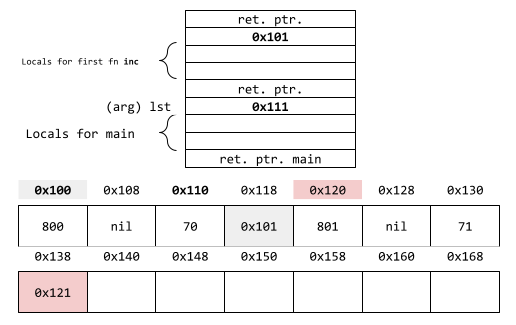
\includegraphics[scale=0.7]{assets/stackHeapPairGC2.png}
\end{center}
The register \code{rax} would have value \code{0x131}. What is considered garbage? The first four words -- \code{0x100} through \code{0x118} -- are considered \textbf{garbage} since there's no references to those words anywhere in the stack. However, why is this the case?  
\begin{itemize}
    \item We'll define the stack as everything at an address higher than \code{rsp} to the top of \code{our\_code\_starts\_here}, but not anything lower address or above that. Therefore, we don't need to consider the following in the stack when deciding what is garbage: 
    \begin{center}
        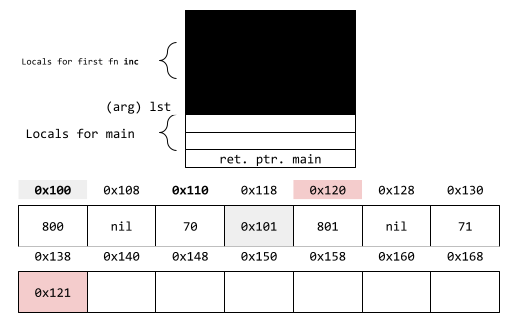
\includegraphics[scale=0.5]{assets/stackHeapPairGC3.png}
    \end{center}

    \item So, as long as no references to \code{0x111} is in main, we can prove that it's garbage.
\end{itemize}
\textbf{Now, let's suppose} our heap only has eight available words. In this example, \code{rax} is \code{0x131}. As one might have suspected, we don't have any memory left to allocate the remaining pairs needed for this program; in particular, after we call the \code{inc} function with the pair that we got from our initial call to \code{inc}, we don't have enough memory to allocate another pair needed for the recursive call. So, we need to collect some garbage. Here's how we might go about this. 
\begin{center}
    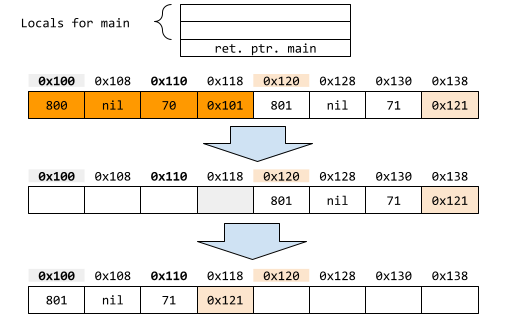
\includegraphics[scale=0.7]{assets/stackHeapPairGCFix4.png}
\end{center}
So, here's what's going on: 
\begin{itemize}
    \item We determined that the first four words are garbage, since no items in the stack or any registers are referring to those four words in the heap. 
    \item We can compact the heap by moving \code{r15} to the beginning of our heap, thus allowing us to reuse the four words that are garbage. 
    \item Now that we have room in the heap, we can allocate the final pair and change \code{rax} to point to our final result.
\end{itemize}
Well, \emph{not quite}. Unlike the previous example, notice how we have a memory address in the heap that's referring to a memory address that's now garbage. That memory address has been relocated, so \textbf{we need to fix this.} Specifically, we need to change the value at \code{0x118} to point to \code{0x100}, not the garbage value at \code{0x120}! Likewise, any call to the stack that uses any memory addresses to the heap might need to be fixed before we can continue. 

\bigskip 

Therefore, we need to not only compact the heap, but also \emph{relocate/forward} all existing references. For this, we will now discuss an algorithm that we can use to perform garbage collection. This algorithm is known as the \textbf{mark-compact algorithm}.

\subsection{Layout and Notation}
In the following sections, we'll make use of the following box to represent heap space. Each square box represents one word in the heap (so each group of boxes represents three words of contiguous heap memory).
\begin{center}
    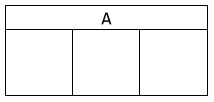
\includegraphics[scale=0.7]{assets/GCAlgLayout.png}
\end{center}
The (A) represents an address to this group of memory (like \code{0x100}).

\bigskip 

The first box of each group is some metadata that we'll need for garbage collection. For our algorithm here, we will need to make use of this metadata. However, there are algorithms out there that don't require metadata.

\bigskip 

In any case, the important thing to remember is that, under this representation, \textbf{each pair} requires 3 words in the heap. 

\subsection{The Algorithm}
At a high level, our algorithm looks like 
\begin{verbatim}
    mark(roots):
        for ref in roots:
            mark_heap(ref)
    
    mark_heap(r):
        if r.marked:
            return 
        r.marked = true 
        for (i, r') in r:
            if ispair(r')
                mark_heap(r')

    fwd_headers():
        from = 0
        to = 0
        while move_from < HEAPEND:
            if from.marked: 
                from.fwd = to 
                to += 3 words/from.size 
            from += 3 words/from.size 
    
    fwd_internal(roots):
        for ref in roots:
            update_fwd(ref)
            fwd_heap(ref)

    fwd_heap(r):
        if r.fwded: 
            return 
        r.fwded = true 
        for (i, r') in r:
            if ispair(r')
                r[i] = getfwd(r')
                fwd_heap(r')

    compact():
        ... \end{verbatim}
Roughly speaking, we can break each of these methods into four groups: 
\begin{enumerate}
    \item \code{mark(roots)} and \code{mark\_heap(r)}
    \item \code{fwd\_headers()}
    \item \code{fwd\_internal(roots)} and \code{fwd\_heap(r)} (forwarding the internal pointers)
    \item Compacting.
\end{enumerate}

\subsection{Motivating Example}
Let's consider the following heap structure.
\begin{center}
    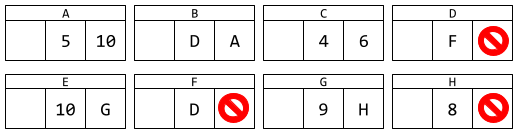
\includegraphics[scale=0.8]{assets/GCAlg1.png}
\end{center}
Note that this example doesn't correspond to any particular program. 

\subsubsection{Step 1: Finding the Root Set}
\begin{mdframed}
    First, we want to find all the references that are currently on the stack (or registers). These are called the \textbf{root set}.
\end{mdframed}
Right now, we don't know what is considered garbage (since we don't know what the stack or the registers look like). So, let's suppose $G$ and $B$ are the only two references on the stack (or registers, depending on implementation). We call this the root set (the roots of your traversal into the heap). Let's suppose we want to \emph{clean} the heap. 

\subsubsection{Step 2: Marking Heap to Find Live Data}
\begin{mdframed}
    Now, we want to call the \code{mark} function with our root set. This is where we're going to \emph{mark} the memory in heap that are still in use (i.e., should not be garbage collected). This process is effectively \underline{depth-first search}.
\end{mdframed}
When we call \code{mark} with our root set, we're iterating over each root, which in our example is $G$ and $B$. 
\begin{itemize}
    \item We first call \code{mark\_heap} with $G$. This will mark $G$, and then recursively call \code{mark\_heap} with $B$ and thus mark $B$ as well. The result of marking is shown below: 
    \begin{center}
        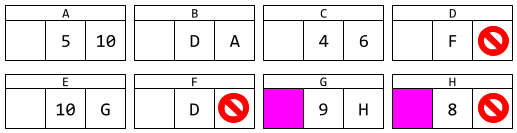
\includegraphics[scale=0.6]{assets/GCAlg2_1.png}
    \end{center}
    Note that we're only considering non-\code{nil} pairs.

    \item Next, we call \code{mark\_heap} with $B$. This will mark $B$, and then  
    \begin{itemize}
        \item recursively call \code{mark\_heap} with $D$, marking it. Then, we'll recursively call \code{mark\_heap} with $F$, marking it. Finally, we recursively call \code{mark\_heap} with $D$, but since this has already been marked we don't need to do anything.
        
        \begin{center}
            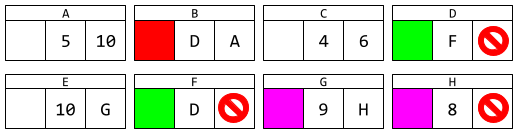
\includegraphics[scale=0.6]{assets/GCAlg2_2.png}
        \end{center}

        \item after that's done, we cal recursively call \code{mark\_heap} with $A$, marking it. Note that, at $A$, there's no other pairs (only raw numbers), so we're done. 
        
        \begin{center}
            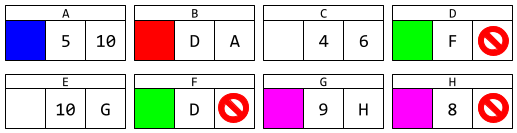
\includegraphics[scale=0.6]{assets/GCAlg2_3.png}
        \end{center}
    \end{itemize}
\end{itemize}
At this point, we're done. Notice how memory (C) and (E) haven't been marked; this means that they're garbage. Our goal, then, is to move \code{r15} to between $F$ and $G$, and start allocation there! This, however, means we need to move everything back (compacting the heap).


\subsubsection{Step 3: Forward Headers}
\begin{mdframed}
    We'll make use of \code{fwd\_headers}. For each marked pair, this function will set the new address (to store that pair after compacting) in the pair's metadata (the first node).
\end{mdframed}

Initially, we'll set \code{move\_to} and \code{move\_from} (\code{to} and \code{from} in the code, respectively) to \code{A} (the first memory location in heap).

\begin{center}
    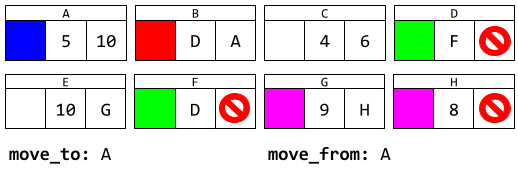
\includegraphics[scale=0.6]{assets/GCAlg3.png}
\end{center}

Iterating over each block of memory, we have 
\begin{enumerate}
    \item Since $\code{move\_from} = A$ is marked, we set its metadata to $\code{move\_to} = A$ (indicating that we'll move $A$ to $A$ after compacting). We also need to increment \code{move\_to} and \code{move\_from}. This gives us the following diagram: 
    \begin{center}
        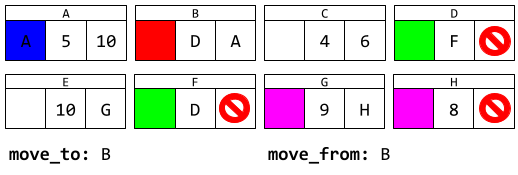
\includegraphics[scale=0.6]{assets/GCAlg3_1.png}
    \end{center}

    \item Since $\code{move\_from} = B$ is marked, we set its metadata to $\code{move\_to} = B$. We also need to increment \code{move\_to} and \code{move\_from}. This gives us the following diagram: 
    \begin{center}
        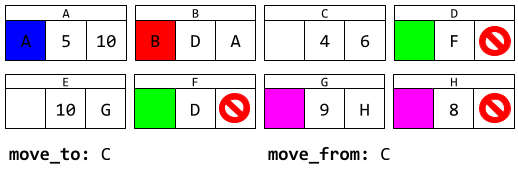
\includegraphics[scale=0.6]{assets/GCAlg3_2.png}
    \end{center}

    \item Since $\code{move\_from} = C$ is \textbf{not} marked, we only increment \code{move\_from}. This gives us the following diagram: 
    \begin{center}
        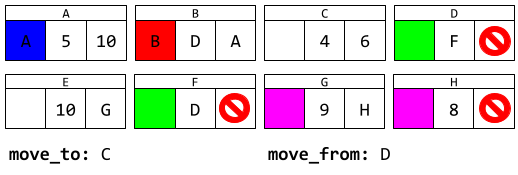
\includegraphics[scale=0.6]{assets/GCAlg3_3.png}
    \end{center}

    \item Since $\code{move\_from} = D$ is marked, we set its metadata to $\code{move\_to} = C$ (indicating that, after compacting, $D$ should be moved to $C$'s location). We also need to increment \code{move\_to} and \code{move\_from}. This gives us the following diagram: 
    \begin{center}
        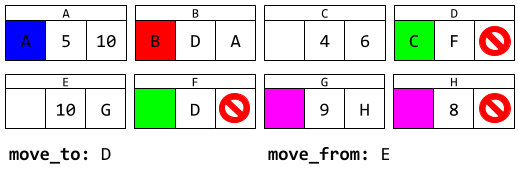
\includegraphics[scale=0.6]{assets/GCAlg3_4.png}
    \end{center}

    \item Since $\code{move\_from} = E$ is not marked, we only increment \code{move\_from}. This gives us the following diagram: 
    \begin{center}
        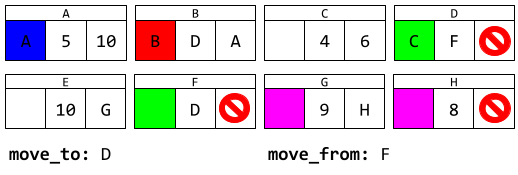
\includegraphics[scale=0.6]{assets/GCAlg3_5.png}
    \end{center}

    \item Since $\code{move\_from} = F$ is marked, we set its metadata to $\code{move\_to} = D$ (indicating that, after compacting, $F$ should be moved to $D$'s location). We also need to increment \code{move\_to} and \code{move\_from}. This gives us the following diagram: 
    \begin{center}
        \includegraphics[scale=0.6]{assets/GCAlg3_6.png}
    \end{center}

    \item Since $\code{move\_from} = G$ is marked, we set its metadata to $\code{move\_to} = E$. We also need to increment \code{move\_to} and \code{move\_from}. This gives us the following diagram: 
    \begin{center}
        \includegraphics[scale=0.6]{assets/GCAlg3_7.png}
    \end{center}

    \item Since $\code{move\_from} = H$ is marked, we set its metadata to $\code{move\_to} = F$. We also need to increment \code{move\_to} and \code{move\_from}. This gives us the following diagram: 
    \begin{center}
        \includegraphics[scale=0.6]{assets/GCAlg3_8.png}
    \end{center}
\end{enumerate}
At this point, we're done. So, we know where each memory location should be moved to after compactness so that the heap is contiguous. \emph{However}, we still need to update all the internal references within the heap!

\subsubsection{Step 4: Forward Internal Addresses}
\begin{mdframed}
    Now that we've marked where everything should be moved to so we can maintain a contiguous heap structure, we still need to update all internal references so they point to the right places. For this, we'll use \code{fwd\_internal}. The idea is that, for each block of memory, we want to consider each reference that the block has, if any. For each reference $r$: 
    \begin{itemize}
        \item Access the original memory block (before compacting) at $r$.
        \item Get its forwarding address and use that as the new reference.
    \end{itemize}
\end{mdframed}
At the moment, this is what our memory diagram looks like: 
\begin{center}
    \includegraphics[scale=0.5]{assets/GCAlg4.png}
\end{center}
\begin{enumerate}
    \item $A$ has no internal references; there's no changes that need to be made. 
    \item One of $B$'s references need to change. 
    \begin{itemize}
        \item Consider reference $D$. Looking up reference $D$, we see that its forwarding address is $C$. Therefore, we replace $D$ with $C$. 
        \item Consider reference $A$. Looking up reference $A$, we see that its forwarding address is $A$. Therefore, we can keep this as $A$. 
    \end{itemize}
    \item $C$ is garbage, so we don't need to consider it. 
    \item For $D$, one of its references need to change. 
    \begin{itemize}
        \item Consider reference $F$. Looking up reference $F$, we see that its forwarding address is $D$. Therefore, we replace $F$ with $D$ here. 
        \item \code{nil} is kept the same. 
    \end{itemize}
    \item $E$ is garbage, so we don't need to consider it. 
    \item One of $F$'s references need to change. 
    \begin{itemize}
        \item Consider reference $D$. Looking it up, we see that its forwarding address is $C$. So, we replace $D$ with $C$.
        \item \code{nil} is kept the same.
    \end{itemize}
    \item One of $G$'s references need to change. 
    \begin{itemize}
        \item 9 is a number, so we leave it alone. 
        \item Consider reference $H$. Looking it up, we see that its forwarding address is $F$. So, we replace $H$ with $F$. 
    \end{itemize}
    \item $H$ has no internal references, so no changes needed.
\end{enumerate}
The result of changing the internal references is 
\begin{center}
    \includegraphics[scale=0.5]{assets/GCAlg4_1.png}
\end{center}

% more implementation at 28:50

\subsubsection{Step 5: Compacting the Heap}
\begin{mdframed}
    Finally, we want to compact the heap. Compacting will be \emph{iteration} (like \code{fwd\_headers}), \textbf{not} traversal (like \code{mark}). In particular, iteration involves iterating over each live data and copying it to its forwarding pointer.
\end{mdframed}

In the compacting step, we want to 
\begin{itemize}
    \item copy each live data to the forwarding pointer, and 
    \item un-mark each data.
\end{itemize}
This gives us 
\begin{center}
    \includegraphics[scale=0.6]{assets/GCAlg5.png}
\end{center}
\newpage
\section{Optimization}
In this section, we'll talk more about optimization. 

\begin{definition}{Optimization}{}
    An \textbf{optimization} (for a compiler) is a version that produces programs that evaluate the same answer as the prior version, but are ``better'' on some cost metric.
\end{definition}

\subsection{Examples of Cost Metrics}
Some examples of cost metrics that we might want to improve on include 
\begin{itemize}
    \item \textbf{Time:} How long does it take for the program to run? 
    \item \textbf{Space:} How much process memory does the program use? 
    \item \textbf{Binary Size:} The size of the compiled binary, and the number of instructions.
    \item \textbf{Executed Instructions:} The overall number of instructions executed (compared to the total number of instructions). This is also similar to the number of jumps in the resulting assembly.  
\end{itemize}
\textbf{Remarks:}
\begin{itemize}
    \item The first two metrics -- time and space -- are generally the most important ones. 
    \item We might also care about properties like compile time, extensibility, debuggability, and platform independence, although these are harder to measure.
\end{itemize}

\subsection{High-Level Optimization Suggestions}
Some suggestions for optimizations include 
\begin{itemize}
    \item \textbf{Register Allocation:} Storing values in registers rather than in memory, since access to registers are generally faster than access to memory. 
    \item \textbf{Dead Code Elimination:} Remove code that the compiler can prove will never run.
    \begin{mdframed}
        (Example.) Consider the following code: 
        \begin{verbatim}
            if false 3 4 \end{verbatim}
        Here, we know for sure the \code{3} will never execute.
    \end{mdframed}
    This also includes things like removing unused variables from compilation. 

    \item \textbf{Constant Folding:} Evaluate ``what you can solve'' in the compiler. 
    \begin{mdframed}
        (Example.) Consider the following code:
        \begin{verbatim}
            (+ (* 2 3) input)\end{verbatim}
        Here, we know that \code{(* 2 3)} should be \code{6}, so this is basically equivalent to 
        \begin{verbatim}
            (+ 6 input)\end{verbatim}
    \end{mdframed}

    \item \textbf{Common Subexpression Elimination:} Eliminate repeated code in favor of a single instance of it. 
    \item \textbf{Memory Packing:} Eliminate unused memory due to alignment (e.g., struct alignment).
    \item \textbf{Loop Unrolling:} We can unroll a loop if we know that it has a constant bound. In other words, essentially hardcode all iterations.
    \begin{mdframed}
        (Example.) Consider the following code: 
        \begin{verbatim}
            (let (x 0) (loop (if (< x 3) (set! x (add1 x)) (break x))))\end{verbatim}
        This is equivalent to  
        \begin{verbatim}
            (let (x 0) (block 
                (set! x (add1 x))
                (set! x (add1 x))
                (set! x (add1 x))
            ))\end{verbatim}
    \end{mdframed}

    \item \textbf{Type-Directed Compilation:} We can remove some code that involves type checking if we know for sure that we're working with the correct types. 
    \begin{mdframed}
        (Example.) Consider the code 
        \begin{verbatim}
            (+ 1 (* input 2))\end{verbatim}
        While type checking is necessary for \code{(* input 2)}, it's probably not necessary for the plus expression since we can assume that both sides are numbers.
    \end{mdframed}

    \item \textbf{Peephole Optimization:} We can remove redundant move operations in the resulting assembly. 
    
    \item \textbf{Inlining Functions:} We can inline function calls, especially if we have a small one. 
    \begin{mdframed}
        (Example.) Consider the following function and resulting code: 
        \begin{verbatim}
            (fun (f x)
                <body>)
            (f 10)\end{verbatim}
        This could be functionally equivalent to  
        \begin{verbatim}
            (let (x 10) <body>)\end{verbatim}
    \end{mdframed}
    Note that we might need to consider things like recursion or other function calls in the function body, since that might prevent us for optimizing. 

    \item \textbf{Instruction Selection:} We can also possibly exploit the structure of our code. 
    \begin{mdframed}
        (Example.) Consider the following code: 
        \begin{verbatim}
            (if (< x 10) ... ...)\end{verbatim}
        Generally, our compiler would put either \code{true} or \code{false} into \code{rax}, and then evaluate \code{rax} when deciding where to jump. However, in this particular code, we can probably just conditionally jump on the spot.  
    \end{mdframed}
\end{itemize}

\subsection{Optimization: Register Allocation}
Let's consider the following code: 
\begin{verbatim}
    (let (n (+ 5 9))
        (let (m (+ 2 3))
            (let (x (+ n 1))
                (let (y (+ m 2))
                    (+ x y)))))\end{verbatim}

The corresponding assembly\footnote{With tag checks removed to make the assembly more concise.}, along with the corresponding code from the above, is shown below.
\begin{verbatim}
    sub rsp, 40
      mov rax, 10
      mov [rsp + 0], rax    ; LHS of (+ 5 9)
      mov rax, 18
      add rax, [rsp + 0]

      mov [rsp + 0], rax    ; Variable n in (let (n ...))

      mov rax, 4
      mov [rsp + 8], rax    ; LHS of (+ 2 3)
      mov rax, 6
      add rax, [rsp + 8]

      mov [rsp + 8], rax    ; Variable m

      mov rax, [rsp + 0]    ; Variable n lookup 
      mov [rsp + 16], rax   ; LHS of (+ n 1)
      mov rax, 2
      add rax, [rsp + 16]

      mov [rsp + 16], rax   ; Variable x

      mov rax, [rsp + 8]    ; Variable m lookup 
      mov [rsp + 24], rax   ; LHS of (+ m 2)
      mov rax, 4
      add rax, [rsp + 24]

      mov [rsp + 24], rax   ; Variable y 

      mov rax, [rsp + 16]   ; Variable x lookup 
      mov [rsp + 32], rax
      mov rax, [rsp + 24]   ; Variable y lookup 
      add rax, [rsp + 32]
    add rsp, 40\end{verbatim}
One thing to notice immediately is that we reused some memory locations. One example is \code{[rsp + 8]}, which is where we stored both a temporary for addition and a value associated with a variable. We can generalize how many memory locations we ultimately \emph{will} use by using the \code{depth} function. In particular, if $\code{depth(expr)} \leq \text{Available Registers}$, then we can avoid memory entirely.

\bigskip 

There are two questions we should now consider.
\begin{enumerate}
    \item (\code{x86\_64}.) What registers should we use?
    \begin{mdframed}
        We can use the registers \code{rbx}, \code{r12}, \code{r13}, \code{r14}, which are callee-saved registers. Note that we aren't using \code{r15} because this register is specifically the heap pointer.
    \end{mdframed}
    \item (Design.) How should we implement this?
    \begin{mdframed}
        We can create a \code{Loc} \emph{enum} that holds either a register or a stack location (offset). Then, our environment can be represented by \code{HashMap<String, Loc>}.

        \bigskip 

        Suppose we have a list of registers that we can use. We can create a \code{get\_loc} function which takes a stack index and returns the new location to be used; this might look something like 
        \begin{verbatim}
    let regs = [...];
    get_loc(si):
        if si < regs.size():
            return regs[si];
        else:
            return Stack(si - regs.len());\end{verbatim}
        Then, we can use this location to update the environment, like 
        \begin{verbatim}
    ... 
    | ELet(x, val, body) => {
        env.update(x, get_loc(si));
    }\end{verbatim}
        Note that, while this is an \emph{improvement} to how our program is compiled, this can still be made a \emph{lot better}. Some other implementation notes to consider include: 
        \begin{itemize}
            \item We need to add code to save and restore registers in function definitions.
            \item We need to compute stack size based on \code{depth - available registers}.
        \end{itemize}
        Some improvements we could make to what we have so far include 
        \begin{itemize}
            \item Registers for outer bindings and stack for inner bindings. 
            \item Frequency matters. 
            \item Precompute registers and locations for all variables and temporaries across functions. 
            \item Are we using the minimal number of locations? (e.g., is the depth minimal?)
        \end{itemize}
    \end{mdframed} 
\end{enumerate}
\textbf{Remark:} The register allocation algorithm we're talking about, which uses an idea similar to \code{depth}, is similar to the \emph{Sethi-Ullman algorithm}.

\subsubsection{High Level Steps}
At a high level, we aim to answer the following questions:
\begin{itemize}
    \item The first step is to find the minimal number of locations needed to store all the working variables in an expression.
    \item What pairs of variables must be stored (or must be ``live'') at the same time? 
\end{itemize}

\subsubsection{The Minimal Number of Locations}
Consider the following program: 
\begin{verbatim}
    (let (b 4)
        (let (x 10)
            (let (i (if input 
                        (let (z 11) (+ z b))
                        (let (y 9) (+ y 1))))
                (let (a (+ i 5))
                    (+ a x)))))\end{verbatim}
To answer the second question, note that 
\begin{itemize}
    \item \code{i} and \code{x} need storage at the same time.
    \item \code{a} and \code{b} do not need storage at the same time\footnote{Notice how we only use \code{b} once: in the \code{if}-expression. After that, we don't use \code{b} again.}. 
\end{itemize}
How many memory locations are needed? We'll look at the program from the \emph{end} to the beginning.
\begin{itemize}
    \item We first begin by looking at what variables are in use at the end. In this case, \code{a} and \code{x} are in use. The set of all variables in use is \[\{a, x\}.\]
    \item We're going to go back ``up'' the program. When we get to a \code{let}-bindings, we're going to remove it from the set of variables that are in use right now. In the next level, we're \emph{using} \code{i} and \code{x}, but we aren't using \code{a} here since \code{a} is being created. The set of all variables in use is \[\{i, x\}.\]
    \item The \code{if}-expression is more interesting. We need to consider both branches of the \code{if}-expression. Note that, in this step, \code{i} is being created, so we don't have access to \code{i} yet.
    \begin{itemize}
        \item Looking at the end of the ``else'' branch, at the body of the \code{let} binding, notice how \code{y} is being used. \code{x} is still around. The set of all variables in use is \[\{y, x\}.\]
        \item Looking at the end of the ``then'' branch, at the body of the \code{let} binding, notice how \code{z} and \code{b}\footnote{Even though \code{b} is defined at the top, this is the first time we're seeing \code{b} in use.} are in use. As usual, \code{x} is still around. The set of all variables in use is \[\{z, b, x\}.\]

    \end{itemize}
    \item At the \code{let}-binding for \code{i} (\emph{not} in the body), we no longer have \code{z} or \code{y}, and \code{i} is being initialized here (so we aren't using \code{i} here). Thus, this gives us the variables in use \[\{x, b\}.\] 
    \item Moving ``up'' the program to the \code{let}-binding for \code{x}, we now only have the variables in use $\{x\}$. 
    \item Finally, moving ``up'' the program to the \code{let}-binding for \code{b}, we have the variables in use $\emptyset$. 
\end{itemize}
This information is telling us what variables need to be stored at the same time. Something we can do with this information is turn this into a \textbf{graph} where there's an edge between two variables \emph{if} they're in use at the same time. 
\begin{center}
    \includegraphics[scale=0.6]{assets/loc_use1.png}
\end{center}
This is a graph where if there are two variables that had to be live at the same time, then there is an edge. How do we make it so we can have a set of locations where each variable can be assigned to a register that's different from all the things it conflicts with? This problem is known as \textbf{graph coloring}. The idea is that we want to find $k$ colors assigning $1 \hdots k$ to each node such that $k$ is minimal and no edge has the same index for both nodes. A coloring for this graph is 
\begin{center}
    \includegraphics[scale=0.6]{assets/loc_use2.png}
\end{center}
We only need 3 colors! In terms of what our compiler would output, we would end up with the environment 
\begin{verbatim}
    {x: 1, b: 2, y: 2, a: 2, z: 3, i: 3}\end{verbatim}
In other words, \code{x} gets abstract location 1, \code{b} gets abstract location 2, and so on. Note that this makes a few assumptions: 
\begin{itemize}
    \item All intermediates are carefully named and used (no useless temporaries).
    \item Assuming all temporaries are explicit, this could replace \code{depth(e)}. Note that this means \emph{simple constants!}
    \item All variables are distinctly named (although we can rename all non-distinct names if needed).
\end{itemize}

\subsubsection{Algorithm}
The algorithm for this process is as follows: 
\begin{itemize}
    \item Visit last, or innermost, expression first. THis means recurse, then working with result. 
    \item Track set of variables we have seen used, then remove from set at the let-bindings.
\end{itemize}
So, going back to the example code, we have the following set of active variables.
\begin{verbatim}
    (let (b 4)                                  ; {}
        (let (x 10)                             ; {b}
            (let (i (if input                   ; {b, x}
                        (let (z 11) (+ z b))    ; {z, b, x}
                        (let (y 9) (+ y 1))))   ; {y, x}
                (let (a (+ i 5))                ; {i, x}
                    (+ a x)))))                 ; {a, x}\end{verbatim}
For each pair of active variables that appear at the same time, we draw an edge between them in the graph.

\subsubsection{Restrictions}
One of the main restrictions of the algorithm for register allocation is simply temporary values: what do we do with register allocation for temporary values that don't have any names?

\subsection{Intermediate Representation}
Let's consider the following program:
\begin{verbatim}
    (+ (- 5 input) (* input (if (> 0 input) 1 -1)))\end{verbatim}
Below is a transformed version of the program where every nested expression that would have introduced a temporary is now a \code{let}-bound variable. 
\begin{verbatim}
    (let (tmp 1 (- t input))
        (let (tmp 2 (> 0 input))
            (let (tmp3 (if tmp2 1 -1))
                (let (tmp4 (* input tmp3))
                    (+ tmp1 tmp4)
                )
            )
        )
    )\end{verbatim}
This makes the order of operations very explicit. Notice that it's very clear that we're doing left-to-right operation. This process also makes code generation for operations a lot easier, since everything is already stored on the stack or in a register. 

\begin{mdframed}
    (Example.) Perform the transformation on the function 
    \begin{verbatim}
    (fun (sumsquares x y)
        (+ (* x x) (* y y)))\end{verbatim}

    \begin{mdframed}
        As mentioned, we want to break our complex expression into much simpler types. We can accomplish this by defining any computations into \code{let}-bindings. This gives us 
        \begin{verbatim}
    (fun (sumsquares x y)
        (let (val (* x x))
            (let (val2 (* y y))
                (+ val val2)
            )
        )
    )\end{verbatim}
    \end{mdframed}
\end{mdframed}
This transformation is fairly common, and there is a fairly standard algorithm for this transformation that takes every non-trivial or non-atomic (basically, everything that's not a literal value) and puts them in a \code{let}-binding. 

\subsubsection{Different Grammar Forms}
There are two types of grammars we want to consider. 
\begin{itemize}
    \item \textbf{A-Normal Form:} This is essentially our grammar as is. This cares about scope, binding, order or evaluations, and so on. 
    
    \begin{verbatim}
        <expr> := <number> | <id> | true | false | nil 
            | (+ <expr> <expr>)
            | (- <expr> <expr>)
            | (if <expr> <expr> <expr>)
            | (break <expr>)
            | ... 
            | (let (<id> <expr>) <expr>)
            | ... \end{verbatim}
    \item \textbf{ANF-Restricted Grammar:} This grammar is effectively the transformed grammar; that is, given our A-Normal Form, we can transform it into a more restricted version. We'll denote this as \code{AExpr}.
    \begin{verbatim}
        <val> := <number> | <id> | true | false | nil 
        <expr> := (+ <val> <val>) 
            | (pair <val> <val>) 
            | (if <val> <block> <block>)
            | (break <val>)
        <block> := (let (<id> <expr>) <block>)
            | (loop <block>)
            | (break <block>+)
            | ... 
            | <expr>
            | <val>\end{verbatim}
        This is restricted in the sense that the grammar is broken up into three different groups (productions). You have expressions (\code{<expr>}) that form blocks (\code{<block>}). Blocks have expressions in them that can perform calculations; so, we can think of \code{<expr>} as something that performs a calculation of some type (e.g., binary operations, creating a new pair, and so on). All the arguments to these expressions that do calculations must be primitive values or identifiers.  
\end{itemize}
\textbf{Remark:} Loops are an interesting case to think about here. 

\subsubsection{Going from Normal to Restricted}
How do we create an algorithm that transforms code written under one grammar to code written in the restricted grammar? Note that this is a very standard algorithm, so we'll mainly gain some intuition. One choice to make is whether we want to introduce a new \code{enum} for ANF expressions. For example, is it worth it to introduce a bunch of new \code{enum}s like shown below?
\begin{verbatim}
    enum Val {
        VNum,
        VId(String),
        ...
    }

    enum AExpr {
        APlus(...),
        APair(...),
        ... 
    }

    enum Block {
        BLet(...),
        ...
    }\end{verbatim}

In any case, we can write a few functions to facilitate the conversion process.
\begin{itemize}
    \item \verb|anf_to_val(e: &Expr) -> Val|: Converts an A-Normal Expression Form to a literal value under the ANF-Restricted Expression Form.
    \item \verb|anf_to_expr(e: &Expr) -> AExpr|: Converts an A-Normal Expression Form to a computation expression under the ANF-Restricted Expression Form.
    \item \verb|anf_to_block(e: &Expr) -> Block|: Converts an A-Normal Expression Form to a block expression under the ANF-Restricted Expression Form. 
\end{itemize}

\subsubsection{ANF to Value}
Let's suppose we want to implement 
\begin{verbatim}
    fn anf_to_val(e: &Expr) -> Val {
        match e {
            ...
        }
    }\end{verbatim}

\begin{itemize}
    \item For an expression \code{e} like \code{Number(n)}, we can trivially return \code{VNum(n)}.
    \item For an expression \code{e} like \code{Plus(e1, e2)}, this becomes more complicated. This will involve a nested plus expression, and we should return an identifier that we can use later. Note that \code{e1} and \code{e2} may be complicated expressions, but we want them to be \code{Val}s as well. So, we'll probably need to do some recursive calls to ideally break \code{e1} and \code{e2} down into \code{let}-bindings. 
    \begin{verbatim}
        Plus(e1, e2) => {
            let (v1, b1) = anf_to_val(e1);
            let (v2, b2) = anf_to_val(e2);
            // Assume new_label() is a function that returns a new identifier.
            let new_name = new_label(); 
            // This isn't Rust syntax, but basically we want all the bindings from 
            // b1, all the bindings from b2, and our new binding in this vector.
            (VId(new_name), vec![...b1, ...b2, (new_name, APlus(v1, v2))])
        }\end{verbatim}
    Notice how we're returning a tuple. The first element is the identifier that will store the result of the evaluation of this expression. However, we also need to return list of \code{let}-bindings we need to eventually stick in front of \emph{this} identifier in order for it to work (otherwise, the identifier won't be bound). So, we should modify the function return type: 
    \begin{verbatim}
    fn anf_to_val(e: &Expr) -> (Val, Vec<(String, AExpr)>) { ... }\end{verbatim}
\end{itemize}

\subsection{Intermediate Representation}
\subsubsection{Rust AST}
Given what we've just discussed, the Rust representation of A-Normal Form and ANF-Restricted Form might look something like 
\begin{verbatim}
    pub enum AVal {
        Num(i32),
        True,
        False,
        Id(String),
    }

    pub enum AExpr {
        Plus(Box<AVal>, Box<AVal>),
        Eq(Box<AVal>, Box<AVal>),
        Lt(Box<AVal>, Box<AVal>),
        Print(Box<AVal>),
        Set(String, Box<AVal>),
        Call1(String, Box<AVal>),
        Call2(String, Box<AVal>, Box<AVal>),
        Pair(Box<AVal>, Box<AVal>),
        Fst(Box<AVal>),
        Snd(Box<AVal>),
        Break(Box<AVal>),
        Loop(Box<ABlock>),
        If(Box<AVal>, Box<ABlock>, Box<ABlock>),
        Val(Box<AVal>),
    }

    pub enum ABlock {
        Let(String, Box<AExpr>, Box<ABlock>),
        Block(Vec<ABlock>),
        Op(Box<AExpr>),
    }\end{verbatim}

\subsubsection{A Problem With Loops}
Consider the following function:
\begin{verbatim}
    (fun (range low high)
        (let (n high)
            (let (lst nil)
                (loop
                    (if (= n low) (break lst)
                        (block
                            (set! n (+ n -1))
                            (set! lst (pair n lst)))
                    )
                )
            )
        )
    )
\end{verbatim}
Converting the above function, which is written in A-Normal Form, to ANF-Restricted Form, yields:
\begin{verbatim}
    (fun (range low high)
        (let (n high)
            (let (lst nil)
                (loop
                    (let (%t_0 (= n low))
                        (if %t_0 (break lst)
                            (block
                                (let (%t_1 (+ n -1)) (set! n %t_1))
                                (let (%t_2 (pair n lst)) (set! lst %t_2)))
                        )
                    )
                )
            )
        )
    )\end{verbatim}
Note that the \verb|%| identifiers are just the convention we're using for temporaries. Let's now consider all interfering variables, which we can do by considering all variables inside-out. 
\begin{verbatim}
    (fun (range low high)
        (let (n high)           ; low, high
            (let (lst nil)                  ; n, low
                (loop
                    (let (%t_0 (= n low))           ; lst, n, low, t_0
                        (if %t_0 (break lst)        ; n, lst, t_0
                            (block
                                (let (%t_1 (+ n -1)) (set! n %t_1))         ; t_1, n, lst
                                (let (%t_2 (pair n lst)) (set! lst %t_2)))  ; t_2, lst, n
                        )
                    )
                )
            )
        )
    )\end{verbatim}
Notice that we end up with the set of variables $\{\code{n}, \code{low}, \code{lst}, \verb|t_0|, \verb|t_1|, \verb|t_2|, \code{high}\}$. A graph representing this would look like 
\begin{center}
    \includegraphics[scale=0.6]{assets/loc_pt2.png}
\end{center}

\begin{mdframed}
    (Exercise.) How would the graph change if we swapped the order of the \code{set!} lines?

    \begin{mdframed}
        \underline{Suggestion:} Because the last use of \code{lst} would be in the first \code{set!} instead of the last line, there wouldn't be an edge between \code{lst} and \code{t\_1}. 

        \bigskip 

        But, one thing to keep in mind is that the \code{set!} is in a loop. So, \code{lst} needs to be in scope for the remainder of the block statement. Otherwise, a temporary could be assigned to the same register that was being used for \code{lst}. 
    \end{mdframed}
\end{mdframed}
\textbf{Remarks:}
\begin{itemize}
    \item Remember that our algorithm just went from the end to beginning, but now we need to consider what identifiers have been defined outside of the loop. 

    \item The issue with loops is that you have implicit backedges from the last expression in the loop to the beginning of the loop. We don't have names associated with these loops, which makes things difficult since we have names in the first place so we know where everything is. 
\end{itemize}

\subsubsection{A Rewrite of the Grammar}
How do we rewrite our grammar to account for loops? 
\begin{verbatim}
    pub enum Val {
        Num(i32),
        True,
        False,
        Id(String),
    }


    pub enum Expr {
        Plus(Box<Val>, Box<Val>),
        Eq(Box<Val>, Box<Val>),
        Lt(Box<Val>, Box<Val>),
        Print(Box<Val>),
        Call1(String, Box<Val>),
        Call2(String, Box<Val>, Box<Val>),
        Pair(Box<Val>, Box<Val>),
        Fst(Box<Val>),
        Snd(Box<Val>),
        Val(Box<Val>),
    }


    pub enum Step {
        Label(String),
        If(Box<Val>, String, String)
        Goto(String),
        Do(Expr),
        Set(String, Expr)
    }


    pub struct Block {
        pub steps: Vec<Step>,
    }\end{verbatim}
Some things to notice here: 
\begin{itemize}
    \item Rather than expressing our program as loops with breaks, we'll express them as labels and gotos. 
    \item In the \code{if}-condition, the first \code{String} is the label to jump to if the condition is true; the last \code{String} is the label to jump to if the condition is false. 
    \item So, whereas ANF is about scope and temporary variables, this is about control flow. Essentially, we're iteratively getting closer to assembly.
\end{itemize}
Here, we introduce the concept of \textbf{intermediate representation}. With the above new representation, we have the following intermediate representation:
\begin{verbatim}
    range(low,high) {
        n <- high
        lst <- nil
       loop_0:
        %t_0 <- n == low
        if %t_0 thn_3 els_4
       thn_3:
        rax <- lst
        goto end_1
        goto ifend_2
       els_4:
        %t_1 <- pair(n, lst)
        lst <- %t_1
        %t_2 <- n + -1
        n <- %t_2
        rax <- n
        goto ifend_2
       ifend_2:
        goto loop_0
       end_1:
        return rax
    }\end{verbatim}
Note that this is the compiled output of the \code{range} function, not in x86\_64. Some things to note: 
\begin{itemize}
    \item There's no nesting of expressions anymore. There's no notion of labels being inside other labels. 
    \item Lots of IRs have support for functions (including things like function scope, blocks within functions, etc.), but leave the actual calling convention to the language. 
    \item The pipeline we would have is that surface syntax turns into ANF, and then ANF turns into IR. It's possible to do everything in one pass, but it's easier to do it in two passes.
    \item In this example of \code{range}, \code{rax} is now our designated answer variable, and we expect all lines before the \code{return rax} line to store the answer into \code{rax} (similar to what our compiler does right now).
\end{itemize}
With that said, running through the IR representation from last to start, the variables in use are: 
\begin{verbatim}
    range(low,high) {           ; {}
        n <- high               ; n
        lst <- nil              ; n, lst 
       loop_0:                  ; n, lst
        %t_0 <- n == low        ; t_0, n, lst 
        if %t_0 thn_3 els_4     ; t_0, n, lst  
       thn_3:                   ; lst 
        rax <- lst              ; rax, lst 
        goto end_1              ; rax 
        goto ifend_2            ; <empty for now>
       els_4:                   ; n, lst, t_1
        %t_1 <- pair(n, lst)    ; n, lst, t_1
        lst <- %t_1             ; lst, n, t_1
        %t_2 <- n + -1          ; t_2, n 
        n <- %t_2               ; t_2, n 
        rax <- n                ; n, rax 
        goto ifend_2            ; <empty for now>
       ifend_2:                 ; <empty for now>
        goto loop_0             ; <empty for now>
       end_1:                   ; rax 
        return rax              ; rax
    }\end{verbatim}
Any time you reach a \code{goto}, any variables that are used at the jump target are copied over to the \code{goto}. In any case, we should not use this information to construct the graph needed to figure out how many registers we need to allocate. In particular, at these three instructions,
\begin{verbatim}
    %t_2 <- n + -1          ; t_2, n 
    n <- %t_2               ; t_2, n 
    rax <- n                ; n, rax \end{verbatim}
there's no edge between \code{lst} and \code{t\_2}. This means that we could potentially store \code{lst} and \code{t\_2} into the same register, losing a possible important value. So, we need to run this same algorithm over and over until none of the sets change (i.e., when saturation occurs). Running through the algorithm again gives us: 
\begin{verbatim}
    range(low,high) {           ; {}                ; 
        n <- high               ; n                 ; 
        lst <- nil              ; n, lst            ; 
       loop_0:                  ; n, lst            ; 
        %t_0 <- n == low        ; t_0, n, lst       ; 
        if %t_0 thn_3 els_4     ; t_0, n, lst       ; 
       thn_3:                   ; lst               ; 
        rax <- lst              ; rax, lst          ;
        goto end_1              ; rax               ; 
        goto ifend_2            ; <empty for now>   ; n, lst
       els_4:                   ; n, lst, t_1       ; 
        %t_1 <- pair(n, lst)    ; n, lst, t_1       ; 
        lst <- %t_1             ; lst, n, t_1       ; 
        %t_2 <- n + -1          ; t_2, n            ; lst 
        n <- %t_2               ; t_2, n            ; lst 
        rax <- n                ; n, rax            ; lst
        goto ifend_2            ; <empty for now>   ; n, lst
       ifend_2:                 ; <empty for now>   ; n, lst
        goto loop_0             ; <empty for now>   ; n, lst
       end_1:                   ; rax               ; 
        return rax              ; rax               ; 
    }\end{verbatim}
Note that the last column are the variables \emph{added} to the variables mentioned in the second columns. Anyways, after running this algorithm again, we reach saturation -- we don't find any additional variables that need to be added. This gives us a complete graph that we can use to determine what registers can be allocated.

\subsection{Flow Analysis}
Let's consider the following code, 
\begin{verbatim}
    (let (curr lst)
        (let (total 0)
            (loop
                (if (= lst nil) (break total)
                    (block
                    (set! total (+ total (fst lst)))
                    (set! lst (snd lst)))))))\end{verbatim}
How can we use flow analysis to reduce the amount of tag checking generated in the final assembly?

\subsubsection{The \code{check} Instruction}
An idea we want to do is to make tag checks explicit with \code{check} steps: which checks can we remove? One new step we can introduce in the intermediate representation is 
\begin{verbatim}
    check <some bool expr>\end{verbatim} 
The semantics are simple: if the check is true, then everything continues as normal. Otherwise, an error is thrown.
\begin{mdframed}
    (Example.) \code{check sametag(curr, nil)} checks to see if \code{curr} has the same tag as \code{nil}. Something we've incorporated into our compiler is the \code{isnum(x)} and \code{isbool(x)} checks, which checks to see if the expression $x$ is a number or boolean, respectively.
\end{mdframed}
With this said, the corresponding intermediate representation of the above code is 
\begin{verbatim}
sum(lst) {
    start0:     curr <- lst
    start1:     total <- 0
    loop_0:     check sametag(curr, nil)
    loop_1:     %t_0 <- curr == nil
    loop_2:     if %t_0 thn_0 els_0
    thn_0:      rax <- total
    thn_1:      goto end_0
    thn_2:      goto ifend_0
    els_0:      check isnonnilpair(curr)
    els_1:      %t_1 <- fst curr
    els_2:      check isnum(total)
    els_3:      check isnum(%t_1)
    els_4:      %t_2 <- total + %t_1
    els_5:      total <- %t_2
    els_6:      check isnonnilpair(curr)
    els_7:      %t_3 <- snd curr
    els_8:      curr <- %t_3
    els_9:      rax <- curr
    els_10:     goto ifend_0
    ifend_0:    goto loop_0
    end_0:      return rax
}\end{verbatim}
We can use flow analysis to analyze how data flows through a program. We can use this information to identify variables that hold values at different points in the program, and how these values change over time. For our purposes, we wish to use flow analysis to reduce the amount of unnecessary tag checking. Using the \code{check} instruction that was mentioned, we can do just this.

\newpage 
\thispagestyle{noheader}
\newgeometry{left=0.1in,right=0.1in,top=0.2in,bottom=0.5in}
\subsubsection{A Flow Analysis Walkthrough}
The flow analysis we'll do starts from the beginning and goes to the end (this is known as \emph{forward analysis}). The information we'll keep track of are the \emph{potential} tags. Let's analyze each line of the intermediate representation. For each line executed, we consider what possible tag value each variable can represent. The potential tags are \textbf{N}umbers, \textbf{B}ooleans, \textbf{Nil}, and \textbf{P}airs. At any point in the program, each variable can hold a set of these possible types. Let $A = \{N, B, \text{Nil}, P\}$ be the set of all types.

\begin{center}
    \begin{tabular}{p{2.5in}|p{0.48in}|p{0.82in}|p{0.48in}|p{0.48in}|p{0.48in}|p{0.48in}|p{0.48in}|p{0.48in}}
        IR & \code{lst} & \code{curr} & \code{total} & $t_0$ & $t_1$ & $t_2$ & $t_3$ & \code{rax} \\ 
        \hline  
        \hline 
        \verb|start0:  curr <- lst|                 & A & $\to A$  &   &   &   &   &   &   \\
        \hline
        \verb|start1:  total <- 0|                  & A & A  & $\to N$ &   &   &   &   &   \\
        \hline
        \verb|loop_0:  check sametag(curr, nil)|    & A  & $\to \{\text{Nil}, P\}$ & N &   &   &   &   &   \\
        \hline
        \verb|loop_1:  %t_0 <- curr == nil|         & A & $\{\text{Nil}, P\}$ & N & $\to B$ &   &   &   &   \\
        \hline
        \verb|loop_2:  if %t_0 thn_0 els_0|         & A & $\{\text{Nil}, P\}$  & N & B &   &   &   &   \\
        \hline
        \verb|thn_0:   rax <- total|                & A & \{\text{Nil}, P\} & N & B &   &   &   & N \\
        \hline
        \verb|thn_1:   goto end_0|                  & A & \{\text{Nil}, P\} & N & B &   &   &   & N \\
        \hline
        \verb|thn_2:   goto ifend_0|\footnote[100]{}     &    &   &   &   &   &   &   &   \\
        \hline
        \verb|els_0:   check isnonnilpair(curr)|\footnote[101]{}  & A & $\{\text{Nil}, P\} \to P$  & N & B &   &   &   &   \\
        \hline
        \verb|els_1:   %t_1 <- fst curr|            & A & P & N & B & $\to A$ &   &   &   \\
        \hline
        \verb|els_2:   check isnum(total)|          & A & P & $N \to N$ & B & $\to A$ &   &   &   \\
        \hline
        \verb|els_3:   check isnum(%t_1)|           & A & P & N & B & $A \to N$ &   &   &   \\
        \hline
        \verb|els_4:   %t_2 <- total + %t_1|        & A & P & N & B & N & $\to N$  &   &  \\
        \hline
        \verb|els_5:   total <- %t_2|               & A & P & $N \to N$ & B & N & N  &   &    \\
        \hline
        \verb|els_6:   check isnonnilpair(curr)|    & A & $P \to P$ & N & B & N & N  &   &    \\
        \hline
        \verb|els_7:   %t_3 <- snd curr|            & A & P & N & B & N & N  & $\to A$ &   \\
        \hline
        \verb|els_8:   curr <- %t_3|                & A & $P \to A$ & N & B & N & N  & A &   \\
        \hline
        \verb|els_9:   rax <- curr|                 & A & A & N & B & N & N & A & $\to A$ \\
        \hline
        \verb|els_10:  goto ifend_0|                & A & A & N & B & N & N & A & A \\
        \hline
        \verb|ifend_0: goto loop_0|                 & A & A & N & B & N & N & A & A \\
        \hline
        \verb|end_0:   return rax|                  &   &   &   &   &   &   &   &   \\
    \end{tabular}
\end{center}
\textbf{Remarks:}
\begin{itemize}
    \item At (100), we have dead code. So, nothing needs to be filled out.
    \item At (101), we can copy the tag information we have from the \code{goto} instruction which jumps to this line. In this case, we copied this information from the line \code{loop\_2}.
    \item In general, we can copy the information from the \code{goto} to the target label. This is especially important when we have a \code{goto} that goes to a label that's \emph{before} where the \code{goto} occurred.
\end{itemize}
At \code{goto loop\_0}, we now perform a backwards jump back to the label \code{loop\_0} and perform additional forward analysis with the information we found prior to the \code{goto}. These tags are denoted by red.
\begin{center}
    \begin{tabular}{p{2.5in}|p{0.48in}|p{0.82in}|p{0.48in}|p{0.48in}|p{0.48in}|p{0.48in}|p{0.48in}|p{0.48in}}
        IR & \code{lst} & \code{curr} & \code{total} & $t_0$ & $t_1$ & $t_2$ & $t_3$ & \code{rax} \\ 
        \hline  
        \hline 
        \verb|start0:  curr <- lst|                 & A & $\to A$  &   &   &   &   &   &   \\
        \hline
        \verb|start1:  total <- 0|                  & A & A  & $\to N$ &   &   &   &   &   \\
        \hline
        \verb|loop_0:  check sametag(curr, nil)|    & A  & $\textcolor{red}{A} \to \{\text{Nil}, P\}$ & N & \textcolor{red}{$\to B$} & \textcolor{red}{$\to N$}  & \textcolor{red}{$\to N$} & \textcolor{red}{$\to A$} & \textcolor{red}{$\to A$} \\
        \hline
        \verb|loop_1:  %t_0 <- curr == nil|         & A & $\{\text{Nil}, P\}$ & N & $\to B$ & \textcolor{red}{N}  & \textcolor{red}{N} & \textcolor{red}{A} & \textcolor{red}{A} \\
        \hline
        \verb|loop_2:  if %t_0 thn_0 els_0|         & A & $\{\text{Nil}, P\}$  & N & B & \textcolor{red}{N}  & \textcolor{red}{N} & \textcolor{red}{A} & \textcolor{red}{A} \\
        \hline
        \verb|thn_0:   rax <- total|                & A & \{\text{Nil}, P\} & N & B & \textcolor{red}{N}  & \textcolor{red}{N} & \textcolor{red}{A} & $\textcolor{red}{A} \to N$ \\
        \hline
        \verb|thn_1:   goto end_0|                  & A & \{\text{Nil}, P\} & N & B & \textcolor{red}{N}  & \textcolor{red}{N} & \textcolor{red}{A} & N \\
        \hline
        \verb|thn_2:   goto ifend_0|     &    &   &   &   &   &   &   &   \\
        \hline
        \verb|els_0:   check isnonnilpair(curr)|\footnote[102]{}  & A & $\{\text{Nil}, P\} \to P$  & N & B & \textcolor{red}{N}  & \textcolor{red}{N} & \textcolor{red}{A} & \textcolor{red}{A} \\
        \hline
        \verb|els_1:   %t_1 <- fst curr|            & A & P & N & B & $\to A$ &   &   &   \\
        \hline
        \verb|els_2:   check isnum(total)|          & A & P & $N \to N$ & B & $\to A$ &   &   &   \\
        \hline
        \verb|els_3:   check isnum(%t_1)|           & A & P & N & B & $A \to N$ &   &   &   \\
        \hline
        \verb|els_4:   %t_2 <- total + %t_1|        & A & P & N & B & N & $\to N$  &   &  \\
        \hline
        \verb|els_5:   total <- %t_2|               & A & P & $N \to N$ & B & N & N  &   &    \\
        \hline
        \verb|els_6:   check isnonnilpair(curr)|    & A & $P \to P$ & N & B & N & N  &   &    \\
        \hline
        \verb|els_7:   %t_3 <- snd curr|            & A & P & N & B & N & N  & $\to A$ &   \\
        \hline
        \verb|els_8:   curr <- %t_3|                & A & $P \to A$ & N & B & N & N  & A &   \\
        \hline
        \verb|els_9:   rax <- curr|                 & A & A & N & B & N & N & A & $\to A$ \\
        \hline
        \verb|els_10:  goto ifend_0|                & A & A & N & B & N & N & A & A \\
        \hline
        \verb|ifend_0: goto loop_0|                 & A & A & N & B & N & N & A & A \\
        \hline
        \verb|end_0:   return rax|                  &   &   &   &   &   &   &   &   \\
    \end{tabular}
\end{center}

\restoregeometry
\newpage 

\textbf{Remark:}
\begin{itemize}
    \item At (102), note that we're not directly copying $N$ from \code{thn\_1} to \code{els\_0}. Rather, we're copying the tag information from the \code{goto} instruction that jumps to this line. 
\end{itemize}
Let's consider the lines \verb|els_2: check isnum(total)| and \verb|els_6: check isnonnilpair(curr)|. Based on the forward analysis, these two lines of code are useless. Likewise, \verb|els_0: check isnonnilpair(curr)| could be \emph{optimized} (not removed) to check if \code{curr} is \code{nil}.

\subsubsection{In Summary}
In summary, the idea behind flow analysis is that there's really two steps: 
\begin{enumerate}
    \item Do the analysis and gather information 
    \item Rescan the program with that information and change the program to remove/optimize any code as needed. 
\end{enumerate}
The corresponding \textbf{control flow graph} looks like 
\begin{center}
    \includegraphics[scale=0.5]{assets/analysis_flow_graph.png}
\end{center}
At the start, we have a bunch of instructions. This eventually leads to a loop. In the \code{thn} branch, we go straight to the end since we have the dead code. In the \code{els} branch, we eventually get to the \code{ifend} statement where we end up going to the loop.

\thispagestyle{noheader}
\newgeometry{left=0.1in,right=0.1in,top=0.2in,bottom=0.5in}

\subsubsection{Another Flow Analysis Walkthrough}
Consider the following program: 
\begin{verbatim}
    (fun (same_at vec1 vec2 i)
        (= (index vec1 i) (index vec2 i)))\end{verbatim}
We'll perform another flow analysis\footnote{Note that this IR representation was generated by hand.}, again by starting from the beginning and going to the end. The information we'll keep track of are the \emph{potential} tags. Our tags are now slightly more refined; in particular, we now have the set of tags, 
\[\text{tag} := Z | \text{Pos} | \text{Neg} | B | V | \text{Nil}\]
Here, \code{Z} means the number zero, \code{Pos} means positive number, \code{Neg} means negative number. We also have \code{B} for boolean, \code{V} for vector, and \code{Nil} for nil. Once again, we let $A$ represent the set of all possible tags. We also introduce $N = \{Z, \text{Pos}, \text{Neg}\}$ for numbers\footnote{Note that there's no overlaps in this set; we either have negative numbers, positive numbers, and zero.}. 

\begin{center}
    \begin{tabular}{p{2.5in}|p{0.65in}|p{0.65in}|p{1.25in}|p{0.65in}|p{0.65in}|p{0.65in}}
        IR & \code{vec1} & \code{vec2} & \code{i} & $t_0$ & $t_1$ & \code{rax} \\ 
        \hline 
        \verb|start0: check isnonnilvec(vec1)|      & $\to V$ &   &   &   &   &   \\
        \verb|start1: check isnum(i)|               & V &   & $\to N$ &   &   &   \\
        \verb|start2: check i >= 0|                 & V &   & $N \to \{Z, \text{Pos}\}$ &   &   &   \\
        \verb|start3: check i < len(vec1)|          & V &   & $\{Z, \text{Pos}\} \to \{Z, \text{Pos}\}$ &   &   &   \\
        \verb|start4: %t_0 <- vec1[i]|              & V &   & $\{Z, \text{Pos}\}$ & $\to A$ &   &   \\
        \verb|start5: check isnonnilvec(vec2)|      & V & $\to V$ & $\{Z, \text{Pos}\}$ & A &   &   \\
        \verb|start6: check isnum(i)|               & V & V & $\{Z, \text{Pos}\}$ & A &   &   \\
        \verb|start7: check i >= 0|                 & . & . & . & . &   &   \\
        \verb|start8: check i < len(vec2)|          & . & . & . & . &   &   \\
        \verb|start9: %t_1 <- vec2[i]|              & . & . & . & . &   &   \\
        \verb|start10:check sametag(%t_0, %t_1)|    &   &   &   &   &   &   \\
        \verb|start10:rax <- %t_0 == %t_1|          &   &   &   &   &   &   \\
        \verb|return rax|                           &   &   &   &   &   &   \\
    \end{tabular}
\end{center}
Note that, at \code{start7}, at our second pass, we can either reduce this to just checking \code{true}, or just deleting the check altogether.

\subsubsection{Abstract Domains}
We're now incorporating forward analysis with some numeric range analysis. We can call these types of analysis abstract domains. We have seen three different abstract domains for analysis: 
\begin{itemize}
    \item \code{Set<String>} for liveliness analysis (for register allocation).
    \item \code{Dict<String, Set<Tag>>} for forward data analysis. 
\end{itemize}
There were two different types of tags: 
\begin{itemize}
    \item \code{Z | P | N}: information about numbers (positive, negative, etc.)
    \item \code{N | B | Nil | P}: other relevant tag information.
\end{itemize}
How do we unify these domains? We can consider ideas like: 
\begin{itemize}
    \item Frequency for variable use.
    \item Frequency of branches. 
    \item Ranges of numbers. 
    \item Booleans as true or false.
    \item Lengths of vectors (if we have constants, e.g., setting the tag to be the length of the vector).
\end{itemize}

\restoregeometry
\newpage 


\end{document}